% Tesis ITAM CLASS -- version 0.1 (13 - Abr - 2015)
% Clase para las tesis del ITAM
%
% 13 - Abr - 2015 	Victor Martinez 	victor.martinez (at) itam.mx
% LICENSE: Creative Commons SA-BY 3.0
%
%
% Este documento presenta un ejemplo de uso de la plantilla
% El estudiante es libre de modificar este archivo a su gusto
%
\documentclass{docITAM}
\usepackage[utf8]{inputenc}
\usepackage{amsfonts}
\usepackage{amsmath}
%\usepackage{algorithmx}
%\usepackage[spanish,onelanguage]{algorithm2e}
%\RestyleAlgo{boxruled} % Para que los algoritmos los ponga en caja
\usepackage[backend=biber]{biblatex}
\usepackage[paperwidth=17cm, paperheight=22.5cm, bottom=2cm, left=2.5cm, right=2cm, headheight=13.08pt]{geometry}
%\usepackage[group-separator={,}]{siunitx}
\usepackage{numprint}
\usepackage{csquotes}
\usepackage{float}
\usepackage{multirow}
\usepackage{url}
\usepackage{subfig} % For multiple images in a single image
\usepackage[font={footnotesize}, labelfont=bf, textfont=it]{caption}
% To customize captions in floating environments (i.e., images)
% Available sizes: scriptsize, footnotesize, small, normalsize, large, Large

\addbibresource{bibliography.bib} %Imports bibliography file
\bibliography{bibliography.bib}

\title{Tesis de Mario}
\author{Mario Humberto Becerra Contreras}
\degree{MAESTRO EN CIENCIAS EN COMPUTACIÓN}
\advisor{Alfredo Garbuno Iñigo}
\year{2018}

\begin{document}
	\npthousandsep{,}
	\pagenumbering{gobble}
	\maketitle
	\publicationrights


	%!TEX root = ../msc_thesis.tex
%\thispagestyle{empty}
\chapter*{\phantom{Dedication}}

Dedication:

\hfil \textit{Most books at the library will have a dedication page. Normally, this page includes quotes like `For my mother' or `For Lucy who never gave up on me.' A dissertation dedication is the same concept. In this part of the dissertation, the student must use a sentence or a paragraph to dedicate their text. They may want to use the dedication to recognize an individual who inspired them to go to college or someone who helped with the dissertation. Dedicating the dissertation to someone is a way to honor them. After putting so much work into this paper, it is a chance for the student to recognize the people who influenced the process.} \hfil

	%!TEX root = ../msc_thesis.tex
%\thispagestyle{empty}
\chapter*{Agradecimientos}

Quiero agradecer a Alfredo Garbuno por asesorar esta tesis. Sus revisiones, comentarios y sugerencias sin duda ayudaron a mejorar mucho el trabajo aquí presentado.

También a Fernando Esponda, Felipe González y Teresa Ortiz por revisar este documento y actuar como sinodales.

Adicionalmente, a Juan Mármol por sus sugerencias sobre el tema y por su ayuda con Microsoft Azure.

Finalmente, a Carlos Serafín por permitirme correr experimentos en su máquina virtual.




	%%%%%%%%%%%%%%%%%%%%%%%%%%%%%%%%%%%%%%%%%%%%%%
	% ABSTRACT
	%%%%%%%%%%%%%%%%%%%%%%%%%%%%%%%%%%%%%%%%%%%%%%

	\begin{abstract}{spanish}
		Una tesis muy bonita.
	\end{abstract}

	\begin{abstract}{english}
		A very nice thesis.
	\end{abstract}

	\selectlanguage{english}
	\setcounter{page}{1}
	\pagenumbering{roman}

	\tableofcontents
	\listoffigures
	\listoftables
	\newpage

	\pagenumbering{arabic}
	\setcounter{page}{1}

	%%%%%%%%%%%%%%%%%%%%%%%%%%%%%%%%%%%%%%%%%%%%%%
	% CONTENT
	%%%%%%%%%%%%%%%%%%%%%%%%%%%%%%%%%%%%%%%%%%%%%%

	%!TEX root = ../mbc_msc_thesis.tex

\chapter{Introduction}
\label{ch:intro}

This is a very nice intro.


	%%!TEX root = ../mbc_msc_thesis.tex

\chapter{Related work}
\label{ch:related_work}




%%% Local Variables:
%%% mode:latex ***
%%% TeX-master: "../mbc_msc_thesis"
%%% End:

	%!TEX root = ../msc_thesis.tex

\chapter{Theoretical Framework}
\label{ch:theory}

%%%%%%%%%%%%%%%%%%%%%%%%%%%%%%%%%%%%%%%%%%%%%%%%%%%%%%%%%%%%%%%%%%%%%%%%%%%%%%%%%%%%%%%%%%
%%%%%%%%%%%%%%%%%%%%%%%%%%%%%%%%%%%%%%%%%%%%%%%%%%%%%%%%%%%%%%%%%%%%%%%%%%%%%%%%%%%%%%%%%%
%%%
%%%%%%%%%%%%%%%%%%%%%%%%%%%%%%%%%%%%%%%%%%%%%%%%%%%%%%%%%%%%%%%%%%%%%%%%%%%%%%%%%%%%%%%%%%
%%%%%%%%%%%%%%%%%%%%%%%%%%%%%%%%%%%%%%%%%%%%%%%%%%%%%%%%%%%%%%%%%%%%%%%%%%%%%%%%%%%%%%%%%%

\section{Machine learning}

Machine learning is a set of methods used to learn patterns in data, and then use these patterns to make predictions about new unseen data, or to take other decisions \cite{murphy2012machine}. With the amount of data available nowadays, it has become a fruitful and demanded field in many areas. Machine learning has exploded lately mainly thanks to the advanced in computing power, without which most of modern techniques wouldn't be feasible.

Machine learning is usually divided in two areas: supervised learning and unsupervised learning. The former involves building a model to predict a response variable from certain explanatory variables (or covariates); while the latter involves a set of variables without a response: one wishes to learn relationships and structure of the data.

An example of supervised learning is to estimate the income of a home from a set of variables such as zip code, size of home, number of cars they own, etc; and an example of unsupervised learning is to find groups of homes that naturally come up in the data, such that there is high similarity within each group and little between groups. In this work, only supervised learning is presented and studied.

As previously mentioned, in supervised learning we have a response variable denoted as vector $y$ with $n$ elements, and each covariate is denoted by $x^{(k)} \in \mathbb{R}^n$ for $k$ from 1 to $p$. All covariates can be summarized in notation in a single data matrix $X \in \mathbb{R}^{n \times p}$. It is assumed that there exists a relationship between $y$ and $X$, which can be written as

\begin{equation}
  \label{eq:general_learning_model}
  Y = f(X) + \varepsilon
\end{equation}

where $f$ is a fixed but unknown function and $\varepsilon$ is a random error term, independent from $X$ and with zero mean \cite[p.~16]{james2013introduction}. We usually want to estimate function $f$, either prediction or inference, and we do it with an estimate $\hat{f}$ \cite[p.~17]{james2013introduction}.
In this work, we will focus on the prediction goal.
The estimate $\hat{f}$ can be chosen from a wide family of models, such as a linear regression model, a general additive model, a neural network, etc., and the goal is for $\hat{f}$ have as little generalization error as possible. This is done using a training set of data, denoted $\mathcal{L} = \left\{ (x_1, y_1), ..., (x_n, y_n) \right\}$, and an error or loss function that we wish to minimize.

For example, in the linear regression case, it is common to minimize the squared error function

\begin{equation}
  \hat{f} = \argmin_{f \in \mathcal{F}} \frac{1}{n} \sum_{i = 1}^n{ ( y_i - f(x_i) ) ^ 2},
\end{equation}

where $\mathcal{F}$ is the family of functions of the form $f(X) = X\theta$ with $\theta \in \mathbb{R}^p$. Thus, $\hat{f}(X) = X \hat{\theta}$, where $\hat{\theta}$ minimizes the error function.

The linear regression model belongs to a type of methods called \textbf{parametric methods}, in which we first make an assumption about the functional form of $f$, and then train the model by choosing the parameters that minimize a previously selected error function \cite[p.~21]{james2013introduction}. In the case of linear regression, the form of $f$ is assumed to be $f(X) = X\theta$, and the parameters chosen are the elements of the $\hat{\theta}$ vector that minimize the squared error function of the model.

An approach to the estimation of parameters that is different to the concept of error function minimization, and one that is also more general, is the one of \textbf{maximum likelihood estimation}.
This is a probabilistic approach in which we assume certain probability distribution for the data.
In the case of linear regression, if we assume that the error term in \ref{eq:general_learning_model} has a Gaussian distribution such that $\varepsilon \sim \normaldist{0}{\sigma^2}$, then $y_i \sim \normaldist{X \theta}{\sigma^2}$; and if we also assume that the observations $y_i$ for $i$ from 1 to $n$ come from a random sample and are, thus, independent of each other, then the log-probability of the sample is

\begin{equation}
  \label{eq:gaussian_likelihood}
  L(\theta) = \sum_{i = 1}^n \log \normalfunc{y_i}{X \theta}{\sigma^2},
\end{equation}

where $\normalfunc{x_i}{\mu}{\sigma^2}$ denotes the density function of a Gaussian random variable with mean $\mu$ and variance $\sigma^2$. The \textbf{principle of maximum likelihood} states that the values for $\theta$ should be chosen so that the observed probability of the random sample is the highest, i.e., so that they maximize equation \ref{eq:gaussian_likelihood} \cite[p.~31]{friedman2001elements}.
With some algebra, it is fairly easy to see that maximizing equation \ref{eq:gaussian_likelihood} is equivalent to minimizing the squared error loss.

In the case of a binary classification problem, assuming that $y_i$ follows a Bernoulli distribution, such that the probability of $y_i$ of being 1 is $p_i(\theta)$, where $\theta$ is the parameter that indexes the probability, then the likelihood function in this case is $\prod_{i = 1}^n  p_i(\theta)^{y_i}\left(1 - p_i(\theta) \right)^{1 - y_i}$ and thus, the log-likelihood is

\begin{equation}
  L(\theta) = \sum_{i = 1}^n \left[ y_i \log\left( p_i(\theta) \right) + (1 - y_i) \log \left( 1 - p_i(\theta) \right) \right].
\end{equation}

Another approach to the learning problem is the \textbf{Bayesian approach}, in which we first assume a prior distribution on the parameters $\theta$ and we update our knowledge about them with data $X$. That is, we first quantify the knowledge that we may have about $\theta$ using a prior distribution $\prob{\theta}$ and then compute the posterior distribution of $\theta$ given $X$ and $y$ using Bayes' theorem as such

\begin{equation}
  \label{eq:bayes_theorem}
  \prob{\theta | X, y} = \frac{\prob{y | \theta, X} \prob{\theta | X}}{\prob{y | X}} = \frac{\prob{y | X, \theta} \prob{\theta | X}}{\int \prob{y | X, \theta} \prob{\theta | X} d\theta}.
\end{equation}

The posterior distribution represents the knowledge that we have about $\theta$ after we have seen the data and is a compromise between our prior beliefs and the data. The multiplier $\prob{X | \theta}$ is called the likelihood, and is the probability of the data given the parameters.

Since the denominator of equation \ref{eq:bayes_theorem} does not depend on $\theta$ because it is only a normalizing constant, it is just usually described as a proportion

\begin{equation}
  \label{eq:bayes_theorem_prop}
    \prob{\theta | X, y} \propto \prob{y | X, \theta} \prob{\theta | X}.
\end{equation}

This posterior distribution is also used to predict the values of unseen data. Let $x^*$ be a vector of covariates for which we want to make a prediction $\hat{y}^*$, then we use the \textbf{posterior predictive distribution}, defined as

\begin{equation}
  \label{eq:post_pred_dist}
  \prob{y^* | X, y, x^*} = \int \prob{y^* | \theta, x^*} \prob{\theta | X, y} d\theta.
\end{equation}

Note that this posterior distribution is, as it name implies, a distribution; i.e., it is not a single prediction but a whole bunch of predictions, quantified by how likely each value is to be. If we wanted a point prediction $\hat{y}^*$ for $x^*$ then we could take the expected value of the posterior predictive distribution such that

\begin{equation}
  \hat{y}^* = \mathbb{E}_{y^* | X, y, x^*} \left[ \prob{y^* | X, y, x^*} \right].
\end{equation}

There are other possible point estimates such as the median, or the maximum a posteriori (MAP) estimate, but we will not study them in detail.

We can illustrate all these concepts in the context of logistic regression. Suppose that we have $n$ observations of a binary response variable $y \in \left\{0, 1\right\}^n$ and two continuous covariates $x^{(1)}, x^{(2)} \in \mathbb{R}^n$. First, we will a build a linear classifier with the frequentist approach, that is, with the maximum likelihood approach; then, we will transform this into a simple learning problem in which we try to minimize a loss function; and finally, we will see how the Bayesian approach works here.

If we wanted to build a linear classifier from our two covariates, we would run into a problem because the response variable only takes the values $0$ and $1$, and a linear model of the form $\mu(x_i) = \theta_0 + \theta_1 x_i^{(1)} + \theta_2 x_i^{(2)}$ is not bounded, so it is a better idea to model the probability of a feature vector of belonging to each class.
This way, $y_i$ is a random variable that follows a Bernoulli distribution with parameter $p_i$, where $p_i$ is the probability of $y_i$ being 1.
The range of $f$ as a linear model is $\mathbb{R}$, so we must map it to the $\left[ 0,1 \right]$ space in which probabilities live, and it can be done with what is called a \textbf{link function}. The \textbf{logistic sigmoid function} $\sigma \left( \cdot \right)$ is a widely used link function for this type of problems \cite[p.~114]{christopher2006pattern}. It is defined as

\begin{equation}
  \sigma(w) = \frac{e^w}{1 + e^w} = \frac{1}{1 + e^{-w}}.
\end{equation}

It is easy to see that $\lim_{w \to -\infty} \sigma(w) = 0$ and $\lim_{w \to \infty} \sigma(w) = 1$. There is more reasoning behind the logistic sigmoid function, and some of it has to be that it belongs to the exponential family of functions. To see more details about this, see \cite{christopher2006pattern}.

Another possible link function is the \textbf{probit function}, defined as the inverse of the cumulative distribution function of a Gaussian random variable \cite[p.~296]{friedman2001elements}. That is, $\sigma(w) = \Phi^{-1}\left( x \right)$,
where

\begin{equation}
  \Phi(w) = \int_{-\infty}^w \frac{1}{\sqrt{2 \pi}} \exp{\left( -\frac{x^2}{2} \right)} dx
\end{equation}

is the Gaussian cumulative distribution function. There are some differences in the theory and behavior of the logistic and the probit functions, but in practice they hardly make any substantial difference. Henceforth, we will use the logistic function as a link function for binary classification problems.

So, we know that $\sigma \left( \cdot \right)$ maps from $\mathbb{R}$ to $\left[ 0,1 \right]$, but we don't know exactly how to relate this to our original problem which is to build a linear classifier using the vectors $x^{(1)}$ and $x^{(2)}$. Using  $\sigma \left( \cdot \right)$, we can define the probability of $y_i$ of belonging to class $1$ given features $x_i^{(1)}$ and $x_i^{(2)}$, summarized as $x_i$, as

\begin{equation}
  \prob{y_i = 1 | x_i, \theta} = \sigma(\theta_0 + \theta_1 x_i^{(1)} + \theta_2 x_i^{(2)}) = \frac{1}{1 + e^{-\left( \theta_0 + \theta_1 x_i^{(1)} + \theta_2 x_i^{(2)} \right)}},
\end{equation}

and thus

\begin{equation}
  \prob{y_i = 0 | x_i, \theta} = 1 - \prob{y_i = 1 | x_i} = \frac{1}{1 + e^{\theta_0 + \theta_1 x_i^{(1)} + \theta_2 x_i^{(2)}}}.
\end{equation}

So, $y_i$ is fully described as a Bernoulli distribution with parameter $p_i =\prob{y_i = 1 | x_i, \theta}$. As we previously mentioned, the likelihood of $n$ observations is

\begin{equation}
  \prod_{i = 1}^n  p_i(\theta)^{y_i}\left(1 - p_i(\theta) \right)^{1 - y_i}
\end{equation}

and, in consequence, the log-likelihood of $n$ observations is

\begin{equation}
  \label{eq:log_likelihood_logistic_example}
  L(\theta) = \sum_{i = 1}^n \left[ y_i \log\left( p_i(\theta) \right) + (1 - y_i) \log \left( 1 - p_i(\theta) \right) \right],
\end{equation}

where $p_i(\theta) = \sigma(\theta_0 + \theta_1 x_i^{(1)} + \theta_2 x_i^{(2)})$.

So, the maximum likelihood estimator of $\theta = \left[ \theta_0, \theta_1, \theta_2 \right]^T$ is the vector $\hat{\theta}$ that maximizes $L(\theta)$ in equation \ref{eq:log_likelihood_logistic_example}; that is $\hat{\theta} = \argmax L(\theta)$.

Another way to see the problem of binary classification, is to simply see it as a learning problem in which we want to minimize a certain loss function. We now know that maximizing equation \ref{eq:log_likelihood_logistic_example} gives us the maximum likelihood estimate, but if we change the sign, then we have a loss function that we can minimize, and it's the exact same problem as before. But first, let's write the new loss function and try to understand the logic behind it. The new objective function, that we wish to minimize is

\begin{equation}
  \label{eq:logistic_example_loss_function}
  L(\theta) = - \sum_{i = 1}^n \left[ y_i \log\left( p_i(\theta) \right) + (1 - y_i) \log \left( 1 - p_i(\theta) \right) \right].
\end{equation}

Now, why is this an error function? If $y_i = 1$, then $1 - y_i = 0$, so the second term in the loss function vanishes and we have remaining $\log\left( p_i(\theta) \right)$. Now, if we assign a high value to $p_i(\theta)$, that is, close to 1, then $\log\left( p_i(\theta) \right) \approx 0$; but if we assign a low value to $p_i(\theta)$, that is, close to 0, then $\log\left( p_i(\theta) \right) \approx -\infty$, and so the overall loss function (don't forget that there's a minus sign at the beginning) tends to infinity. This means that when the real value of $y_i$ is 1 and we assign a low probability to it, the loss function is large, but if we assign a high probability to it, the loss function is small. The same reasoning works for when $y_i = 0$: if we assign a low probability, then the loss function is small, but if we assign a high probability, then the loss function is large. Hence, minimizing the loss function leads to choosing values of $\theta$ such that they yield a high probability to the cases when $y_i = 1$ and a low one when $y_i = 0$.

% There are other possible loss functions for this problem, such as the \textbf{hinge loss}

Now, let's move to the Bayesian approach to logistic regression. As before, we will assume that $y_i$ follows a Bernoulli distribution such that the probability of being 1 is $p_i(\theta) = \sigma(\theta_0 + \theta_1 x_i^{(1)} + \theta_2 x_i^{(2)})$, with $\sigma \left( \cdot \right)$ the logistic sigmoid function. In the Bayesian paradigm, parameter vector $\theta = \left[ \theta_0, \theta_1, \theta_2 \right]^T$ must have a joint prior distribution. As mentioned before, a good idea is to place a Gaussian distribution to it and, in this case, assume independence between the parameters, such that

\begin{equation}
  \theta \sim \normaldist{\mu}{\frac{1}{\tau} I}
\end{equation}

where $\mu \in \mathbb{R}^3$, $\tau \in \mathbb{R}^+$ and $I$ is a $3 \times 3$ identity matrix. In this context, $\tau$ is the inverse of the variance, and is called the \textbf{precision}. Assuming $\mu = \left[ \mu_0, \mu_1, \mu_2 \right]^T$, then the prior distribution takes the following form

\begin{equation}
  \prob{\theta} = \prod_{k = 0}^2 \sqrt{\frac{\tau}{2 \pi}} e^{- \tau \frac{\left( \theta_k - \mu_k \right)^2}{2}}.
\end{equation}

And, the likelihood is

\begin{equation}
  \prob{X | \theta} = \prod_{i = 1}^n  p_i(\theta)^{y_i}\left(1 - p_i(\theta) \right)^{1 - y_i},
\end{equation}

so, following Bayes' theorem in equation \ref{eq:bayes_theorem_prop}, the posterior distribution is

\begin{equation}
  \prob{\theta | X, y} =
    \frac
    {
      \left[ \prod_{i = 1}^n  p_i(\theta)^{y_i}\left(1 - p_i(\theta) \right)^{1 - y_i} \right]
      \left[ \prod_{k = 0}^2 \sqrt{\frac{\tau}{2 \pi}} e^{- \tau \frac{\left( \theta_k - \mu_k \right)^2}{2}} \right]
    }{
      \int \left[ \prod_{i = 1}^n  p_i(\theta)^{y_i}\left(1 - p_i(\theta) \right)^{1 - y_i} \right]
      \left[ \prod_{k = 0}^2 \sqrt{\frac{\tau}{2 \pi}} e^{- \tau \frac{\left( \theta_k - \mu_k \right)^2}{2}} \right] d\theta
    }.
\end{equation}

Unfortunately, the integral is not directly solvable, and that is the reason numerical methods are used. Most of them rely on the fact that the denominator is only a normalizing constant and only use the equation as a proportion

\begin{equation}
  \prob{\theta | X, y} \propto
  \left[ \prod_{i = 1}^n  p_i(\theta)^{y_i}\left(1 - p_i(\theta) \right)^{1 - y_i} \right]
  \left[ \prod_{k = 0}^2 \sqrt{\frac{\tau}{2 \pi}} e^{- \tau \frac{\left( \theta_k - \mu_k \right)^2}{2}} \right].
\end{equation}

Methods to estimate the posterior include Markov Chain Monte Carlo (MCMC) methods such as Metropolis-Hastings or Hamiltonian Monte Carlo, and Variational Inference, discussed later in this document.

No matter what paradigm we choose to follow, in general, when one is training a model for prediction, it is not the main goal to minimize training error, but prediction error; i.e., the error of any future observation $(X^0, Y^0)$. This means that we want to minimize the expected prediction error, hence, we usually divide the data set $(X, Y)$ in two: the training set and the test set. To do this, from the original data set, a random sample of observations is assigned to be part of the training set and the rest are part of the test set.The idea is that the test set should be used to measure the predictive performance of the model. A third set is sometimes added and is called the validation set, in which predictive performance is measured to select certain hyperparameters, such as regularization parameter values, discussed further in this document.


%%%%%%%%%%%%%%%%%%%%%%%%%%%%%%%%%%%%%%%%%%%%%%%%%%%%%%%%%%%%%%%%%%%%%%%%%%%%%%%%%%%%%%%%%%
%%%%%%%%%%%%%%%%%%%%%%%%%%%%%%%%%%%%%%%%%%%%%%%%%%%%%%%%%%%%%%%%%%%%%%%%%%%%%%%%%%%%%%%%%%
%%% Loss function optimization
%%%%%%%%%%%%%%%%%%%%%%%%%%%%%%%%%%%%%%%%%%%%%%%%%%%%%%%%%%%%%%%%%%%%%%%%%%%%%%%%%%%%%%%%%%
%%%%%%%%%%%%%%%%%%%%%%%%%%%%%%%%%%%%%%%%%%%%%%%%%%%%%%%%%%%%%%%%%%%%%%%%%%%%%%%%%%%%%%%%%%

\section{Loss function optimization}

As mentioned before, in machine learning one usually wants to find the parameters that minimize a loss function such as the one in equation \ref{eq:logistic_example_loss_function}, a problem which in some cases, as in linear regression, using the first and second order conditions, we can find a closed formula to find the parameters; but in many other cases, such as in logistic regression, this is not possible, so we resort to numerical optimization techniques.
The general problem of unrestricted optimization \cite{nocedal2006numerical} is

\begin{equation}
  \min_{\theta \in \mathbb{R}^p} L(\theta).
\end{equation}


For statistical learning, $L$ is usually a convex loss function and $\theta$ is a parameter or vector of parameters. A solution is a vector $\theta^*$ called local minimizer, which makes the function $L$ to be minimized in a neighborhood around $\theta^*$. Formally, a vector $\theta^*$ is a local minimizer if there exists a neighborhood $\mathcal{N}$ of $\theta^*$ such that $L(\theta^*) \leq L(\theta)$ for all $\theta \in \mathcal{N}$.

In numerical optimization, we make use of the sufficient second order conditions. Suppose that the Hessian matrix $\nabla^2 L$ is continuous in an open neighborhood of $\theta^*$, that the gradient $\nabla L(\theta^*) = 0$ and that $\nabla^2 L(\theta^*)$ is positive definite; then $\theta^*$ is a local minimizer of $L$.

This is basic calculus, but it provides the base of numerical optimization algorithms. In general, all algorithms search for a point $\theta^*$ such that $\nabla L(\theta^*) = 0$.



\subsection{Gradient descent (GD)}

Generally, numerical optimization algorithms are iterative, and gradient descent belongs to this class, particularly, it belongs to a family called \textbf{line search algorithms}. In each iteration, the algorithms search for a direction in which to go and then update the current value in accordance to that direction. That is, in the $k$-th iteration, we have a value $\theta_k$, and we look for a direction $p_k$ to update to a new value $\theta_{k+1} = \theta_k + \alpha_k p_k$, where $\alpha_k > 0$ is the ``distance'' in which the algorithm moves toward direction $p_k$, and is called \textbf{step length}. Once that the value of the parameter is updated, we find a new direction in which to move forward and then update the parameter value again. This is done until a stopping criteria is met, this usually being that the gradient vector norm is smaller than a certain small positive scalar.

In gradient descent, the direction $p_k$ in which the algorithm moves is the maximum descent direction, that is, the negative of the gradient $-\nabla L(\theta_k)$. So, in each iteration we have

\begin{equation}
  \theta_{k+1} = \theta_k - \alpha_k \nabla L(\theta_k).
\end{equation}

We find a problem when we want to compute the step length $\alpha_k$: we want to find a value that the function $L$ decreases as much as possible, but we don't want to waste much time choosing the value. The best option is the global minimizer of the auxiliary function $\phi(\alpha_k) = L(\theta_k + \alpha_k p_k)$, but it is too expensive to compute. Generally, heuristics are used to choose the sequence of values for $\alpha_k$, such as using the outer product of the gradient with itself, as shown in \cite{duchi2011adaptive}.

In the case of logistic regression, we want to minimize loss function defined in equation \ref{eq:logistic_example_loss_function}, which is

\begin{equation}
  L(\theta) = - \sum_{i=1}^{n} \left[ y_i \log(\sigma(\theta^T x_i)) + (1-y_i) \log(1-\sigma(\theta^T x_i)) \right] =
  - \sum_{i=1}^{n}{\ell_i(\theta)}
\end{equation}

where $\sigma(\cdot)$ is the logistic sigmoid function, $\theta^T x_i = \sum_{j=0}^{p}{\theta_j x_{ij}}$ and $\ell_i(\theta)$ is defined as

\begin{equation}
  \ell_i(\theta) = y_i \log(\sigma(\theta^T x_i)) + (1-y_i) \log(1-\sigma(\theta^T x_i)).
\end{equation}

We take the partial derivatives

\begin{equation}
  \frac{\partial L}{\partial \theta_j} = - \sum_{i = 1}^n { \frac{\partial \ell_i}{\partial \theta_j} }
\end{equation}

and, using the fact that $\sigma'(w) = \sigma(w)(1-\sigma(w))$, we have

\begin{equation}
  \begin{split}
    \frac{\partial \ell_i}{\partial \theta_j} & =
    \frac{y_i \sigma'(\theta^T x_i) x_{ij} }  {\sigma(\theta^T x_i)} + \frac{(1 - y_i) (-1) \sigma'(\theta^T x_i) x_{ij}} {1 - \sigma(\theta^T x_i)} \\
    & = \frac{\sigma'(\theta^T x_i) x_{ij} y_i}{\sigma(\theta^T x_i)} - \frac{(1 - y_i) \sigma'(\theta^T x_i) x_{ij}}{1 - \sigma((\theta^T x_i))} \\
    & = \sigma'(\theta^T x_i) x_{ij} \left(\frac{y_i}{\sigma(\theta^T x_i)} - \frac{1-y_i}{1-\sigma(\theta^T x_i)} \right) \\
    & = \sigma'(\theta^T x_i) x_{ij} \left(\frac{y_i - y_i \sigma(\theta^T x_i) -
    \sigma(\theta^T x_i) + y_i \sigma(\theta^T x_i)}{\sigma(\theta^T x_i)(1-\sigma(\theta^T x_i))} \right) \\
    & = x_{ij}(y_i - \sigma(\theta^T x_i)).
  \end{split}
\end{equation}

So, we have that

\begin{equation}
  \frac{\partial L}{\partial \theta_j} = - \sum_{i = 1}^n { x_{ij}(y_i - \sigma(\sum_{j=0}^{p}{\theta_j x_{ij}})) },
\end{equation}

where once more $x_{i1} = 1$ for all $i \in \left\{1, ..., n \right\}$.


From here, we have that the gradient descent direction for each iteration is

\begin{equation}
  \nabla_{\theta} L = \left( \frac{\partial L}{\partial \theta_0}, ..., \frac{\partial L}{\partial \theta_p} \right)^T.
\end{equation}

To minimize the loss function, we start with an initial vector of parameters $\theta^0 \in \mathbb{R}^2$, and in each iteration we update

\begin{equation}
  \theta^{k+1} = \theta^k - \alpha_k \nabla_{\theta} L(\theta)
\end{equation}

until certain criteria are met.

To see this algorithm in action, we can see an implemented example in the R programming language in which we generate a vector $x \in \mathbb{R}^n$ with $n = 1000$ such that $x_i \sim N(0, 1)$ for each $i \in \left\{1, ..., n \right\}$, then an auxiliary vector was computed, $p_i = \frac{1}{\exp \left( - \theta_0 - \theta_1 x_i \right)}$, with $\theta_0 = -5$ and $\theta_1 = 5$. Finally, the response variable $y$ was built simulating Bernoulli random variables, such that $y_i \sim \mathrm{Bern}(p_i)$.
The implementation is compared with the result of the \texttt{glm} package.

The initial vector of parameters was $\theta^0 = (0, 0)^T$ and we used a constant value of $\alpha_k = 2$.The stopping criteria was that the norm of the gradient $\nabla_{\theta} L(\theta)$ should be less than $0.0001$, which was achieved after 409 iterations.

Figure \ref{fig:GD_plots} shows the results of the implementation. On the left, we can see the value of the loss function in each iteration. On the right we can see the parameter vector's value in each iteration. The red dot is the value of the estimate by the \texttt{glm} package. We can see that the implemented algorithm converges to this value.

\begin{figure}[H]
    \centering
    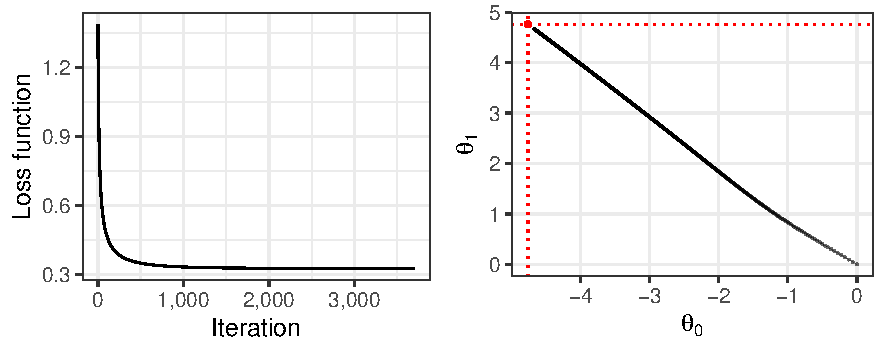
\includegraphics[width=\textwidth]{GD_plots.pdf}
    \caption{Example of gradient descent for logistic regression.}
    \label{fig:GD_plots}
\end{figure}


\subsection{Stochastic gradient descent (SGD)}

In machine learning it is common to find the need to solve optimization problems of the form

\begin{equation}
  \min_{\theta \in \mathbb{R}^p} L(\theta), \quad \text{with} \, \,
  L(\theta) = \frac{1}{n} \sum_{i = 1}^n { \ell_i(\theta) }.
\end{equation}

In the past logistic regression example, the loss function that we wanted to minimize was expressed in that way. Gradient descent uses iterations in the form

\begin{equation}
  \theta_{k+1} = \theta_k - \alpha_k \nabla L(\theta_k) :=\theta_k - \frac{\alpha_k}{n} \sum_{i = 1}^n \nabla \ell_i(\theta_k),
\end{equation}

which involves evaluating $n$ gradients (one for each observation) and then taking an average. In some cases of machine learning, $n$ can be really big; hence computing all of those gradients in each iteration is expensive. That is why researchers come up with methods such as SGD, in which the number of gradients to compute does not depend on $n$ and is constant instead. SGD uses iterations of the form

\begin{equation}
  \theta_{k+1} = \theta_k - \alpha_k \nabla \ell_{i_k}(\theta_k),
\end{equation}

where $i_k \in \left\{1, 2, ..., n \right\}$ is randomly chosen. The gradient $\nabla \ell_{i_k}(\theta_k)$ is an unbiased estimator of $\nabla L(\theta_k)$. This way, each iteration is really cheap because it involves the computation of only one gradient. It can happen that some $\nabla \ell_{i_k}(\theta_k)$ in particular does not give a direction of descent from $\theta_k$, but on average we do get descent directions, such that the sequence $\left\{ \theta_0, \theta_1, ... \right\}$ guides to a minimizer $\theta^*$.

\subsection{Mini-batch gradient descent}

An approach that is in between the two extremes of computing the gradients of all observations and the gradient of just one observation is \textbf{mini-batch gradient descent}. In mini-batch gradient descent, one chooses a fixed integer $l$, then the data set is divided in batches if size $l$, where the values in each batch are randomly chosen. Then, each of these batches is used to compute the gradient and update the values of the parameters. Usually $l$ is a small number compared to the size of a big data set, but big enough so that the gradient estimation is not too noisy, such as $l = 32$ or $l = 100$. This way, each iteration is cheaper because it involves the computation of only $l$ gradients instead of $n$. Stochastic gradient descent (SGD) is just mini-batch gradient descent with $l = 1$.

So, mini-batch gradient descent updates the value of the parameters in each iteration as such


\begin{equation}
  \theta_{k+1} = \theta_k - \frac{\alpha_k}{n} \sum_{i = 1}^l \nabla \ell_i(\theta_k).
\end{equation}


We implemented mini-batch gradient descent for logistic regression in R and test it with the same simulated data set as in the previous example. Figure \ref{fig:Mini-batch_GD_plots} shows the results of the implementation. Each of the plots shows the values of the parameters in each iteration, but the difference in each plot is the size of the mini-batch $l$. It is clear that with bigger $l$, the descent directions are less noisy, but in the end they all converge to more or less the same value.

\begin{figure}[H]
    \centering
    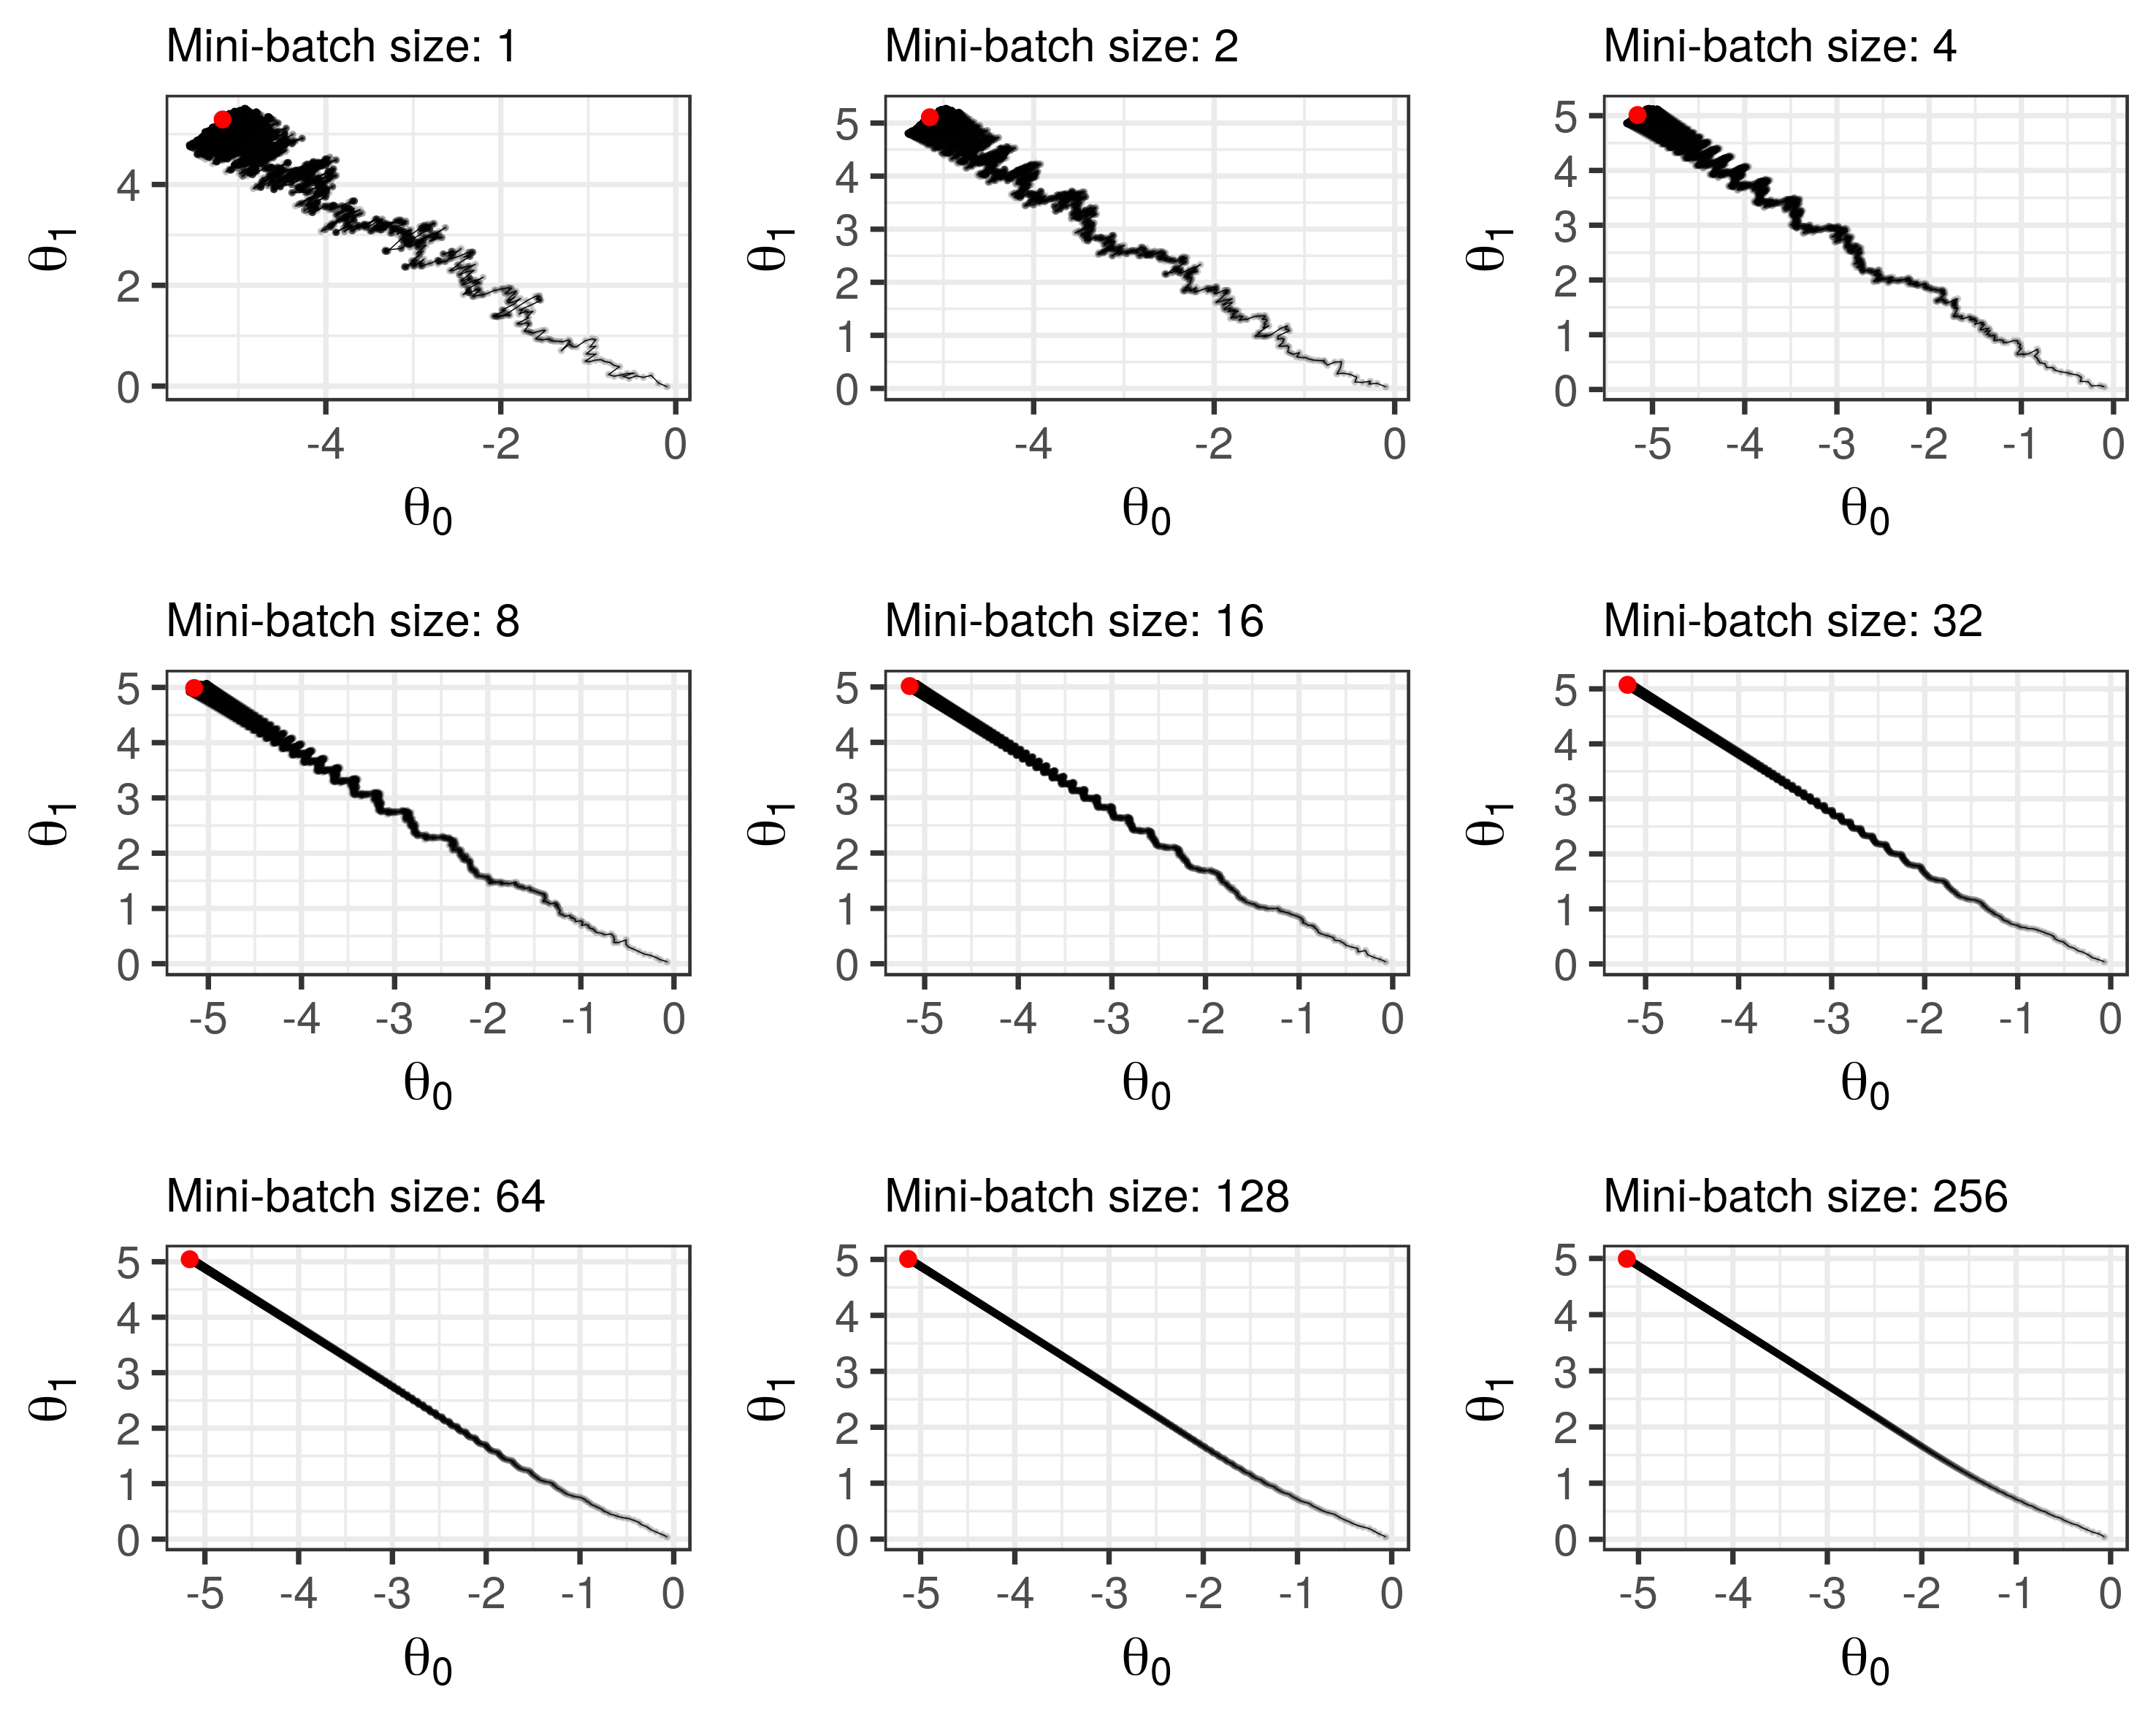
\includegraphics[width=\textwidth]{Mini-batch_GD_plots.png}
    \caption{Example of mini-batch gradient descent for logistic regression comparing mini-batch sizes.}
    \label{fig:Mini-batch_GD_plots}
\end{figure}


\subsection{Overfitting and regularization}

A common problem in machine learning can be \textbf{overfitting}. To explain this, consider the case of modeling a response variable $Y$ with the general model proposed in equation \ref{eq:general_learning_model}. If $f$ is too flexible, then a larger number of parameters must be estimated, which leads to part of the error being captured by those parameters. This is known as overfitting. The problem with an overfit model is that it will give bad predictions with data that has not been previously observed. This is why overfit models have a small training error, but a large test error.

One way to control overfitting is with \textbf{regularization}, in which a penalization term is added to the loss function to prevent the parameters from taking values that are too high. A very simple regularizer is the $L_2$ norm regularizer in which the sum of the squared parameters is added to the loss function.

For example, in linear regression, the usual loss function that we seek to minimize is

\begin{equation}
  \label{eq:lin_reg_loss_funct}
  \sum_{i = 1}^n{ \left( y_i - \sum_{k = 0}^p  \theta_k x_k \right) ^ 2},
\end{equation}

but with the $L_2$ regularizer (also known as ridge regression), equation \ref{eq:lin_reg_loss_funct} is modified so that the loss function now is

\begin{equation}
  \label{eq:lin_reg_loss_funct_reg}
  \sum_{i = 1}^n{ \left( y_i - \sum_{k = 0}^p \theta_k x_k \right) ^ 2}
  + \lambda \left( \sum_{k = 1}^p \theta_k^2 \right),
\end{equation}

where $\lambda > 0$ is called the regularization parameter, and controls the relative importance between the two main terms of the sum. The value of this parameter can have a big impact in the loss function: if it is too big, then it will penalize too much and most parameters will be near 0, but if it is too small, then there is little regularization effect and it is as if there were no penalization at all. In practice, it is common to choose several concrete values of $\lambda$ (such as 0.001, 0.01 and 0.1) and select the final value using the validation set previously mentioned, so that the final $\lambda$ minimizes the validation set error.

Another type of regularization that is widely used in neural network literature nowadays is \textbf{dropout} \cite{srivastava2014dropout}. Dropout consists in randomly dropping out, that is temporarily removing, units of the neural network in each feed-forward mini-batch pass, which results in a thinned network. Each unit is removed, along with all its input and output connections, with a certain probability $p$. The original idea of dropout is that by randomly dropping units, we are essentially training different networks, so the end result is the combination of different architectures, which result in less overfitting. At test time, the prediction is usually just the average of the different thinned networks.

In \citeyear{gal2015dropout1}, \citeauthor{gal2015dropout1} proved that dropout can be seen as a Bayesian approximation to a deep Gaussian process \cite{gal2015dropout}. They show that applying dropout before each weight layer in a neural network with arbitrary depth is mathematically equivalent to a variational approximation that minimized the KL divergence to the posterior distribution to a deep Gaussian process. They later showed that stochastic regularization techniques such as dropout, can be seen as variational approximations to a Bayesian neural network, including convolutional neural networks \cite{gal2015bayesian} \cite{gal2015modern}.


%%%%%%%%%%%%%%%%%%%%%%%%%%%%%%%%%%%%%%%%%%%%%%%%%%%%%%%%%%%%%%%%%%%%%%%%%%%%%%%%%%%%%%%%%%
%%%%%%%%%%%%%%%%%%%%%%%%%%%%%%%%%%%%%%%%%%%%%%%%%%%%%%%%%%%%%%%%%%%%%%%%%%%%%%%%%%%%%%%%%%
%%% VI
%%%%%%%%%%%%%%%%%%%%%%%%%%%%%%%%%%%%%%%%%%%%%%%%%%%%%%%%%%%%%%%%%%%%%%%%%%%%%%%%%%%%%%%%%%
%%%%%%%%%%%%%%%%%%%%%%%%%%%%%%%%%%%%%%%%%%%%%%%%%%%%%%%%%%%%%%%%%%%%%%%%%%%%%%%%%%%%%%%%%%

\section{Variational Inference}

As mentioned before, when doing Bayesian inference, it is of interest to compute the posterior distribution $\prob{\theta | X, y}$, which is very often intractable, so one must resort to numerical approximations. In this section, we'll give a brief overview of one possible numerical approximation, called variational inference (VI). The idea of VI is to use optimization to approximate the target distribution $\prob{\theta | X, y}$ with some other approximate distribution $q(\theta)$ that minimizes the Kullback-Leibler (KL) divergence to the real posterior \cite{blei2017variational}. We will define such divergence as
\begin{equation}
  \label{eq:kl_divergence}
  \kl{q}{p} = \mathbb{E}_q \left[ \log \left( \frac{q(\theta)}{\prob{\theta | X, y}} \right) \right] = \int_{-\infty}^{\infty} q(\theta) \left[ \log \left( \frac{q(\theta)}{\prob{\theta | X, y}} \right) \right] d\theta.
\end{equation}

Note that the KL divergence is not symmetrical, i.e., $\kl{q}{p} \neq \kl{p}{q}$, and that we usually try to minimize $\kl{q}{p}$ instead of $\kl{p}{q}$ because the latter requires averaging with respect to $\prob{\theta | X, y}$, which is what we are trying to approximate in the first place. Methods to deal with this type of KL divergence exist and are called expectation propagation, but they are not of concern in this work.

Although the main goal of VI methods is tho minimize the KL divergence in \ref{eq:kl_divergence}, in practice what is usually done is to maximize a related quantity called the ELBO (Evidence Lower BOund), defined as

\begin{equation}
  \label{eq:elbo_def}
  \mathcal{L}(q) = \mathbb{E}_q\left[ \log p(X, y, \theta) \right] - \mathbb{E}_q\left[ \log q(\theta) \right].
\end{equation}

The relationship between ELBO and KL divergence is easy to see. Starting from the KL divergence definition, using the logarithm quotient rule, and by the fact that the expected value is a linear operator, we have

\begin{equation}
    \kl{q}{p} =
    \mathbb{E}_q \left[ \log \left( \frac{q(\theta)}{\prob{\theta | X, y}} \right) \right] =
    \mathbb{E}_q \left[ \log  q(\theta) \right] - \mathbb{E}_q \left[ \log {\prob{\theta | X, y}}  \right].
\end{equation}

Then, using the definition of conditional probability, we have

\begin{equation}
    %\mathbb{E}_q \left[ \log  q(\theta) \right] - \mathbb{E}_q \left[ \log p(\theta | X, y)  \right] =
    \kl{q}{p} =
    \mathbb{E}_q \left[ \log  q(\theta) \right] - \mathbb{E}_q \left[ \log \frac{p(\theta, X, y)}{p(y | X) p(X)}  \right].
\end{equation}

Using the logarithm quotient rule one more time

\begin{equation}
  % \mathbb{E}_q \left[ \log  q(\theta) \right] - \mathbb{E}_q \left[ \log \frac{p(\theta, X, y)}{p(y | X) p(X)}  \right] =
  \kl{q}{p} =
  \mathbb{E}_q \left[ \log  q(\theta) \right] - \mathbb{E}_q \left[ \log p(\theta, X, y) - \log p(y | X) - \log p(X)  \right].
\end{equation}

But since $p(X)$ does not depend on $q$, the expected value of $p(X)$ is a constant; so we have

\begin{equation}
 %\mathbb{E}_q \left[ \log  q(\theta) \right] - \mathbb{E}_q \left[ \log p(\theta, X) - \log p(X)  \right] =
 \kl{q}{p} =
 \mathbb{E}_q \left[ \log  q(\theta) \right] - \mathbb{E}_q \left[ \log p(\theta, X, y) \right] + \log p(y | X) + \log p(X)
\end{equation}

And since we are trying to find the optimal $q$, then $\log p(X)$ is just a constant in the optimization process, and we can disregard it and just minimize equation

\begin{equation}
  \mathbb{E}_q \left[ \log  q(\theta) \right] - \mathbb{E}_q \left[ \log p(\theta, X, y) \right]
\end{equation}

which as we see, is the negative of the ELBO, so minimizing the KL divergence is equivalent to maximizing the ELBO.

Let $\lambda$ be the parameters of the variational distribution $q(\theta)$. The objective is to approximate $p(\theta | X, y)$ by finding the values of the $\lambda$ vector that maximize equation \ref{eq:elbo_def}, which could be done in several ways, for example, coordinate ascent, or gradient ascent. In order to perform gradient ascent, we need to compute the gradient of the objective function with respect to the parameters, that is, we need $\nabla_{\lambda} \mathcal{L}(q, \lambda)$. It is not very hard to prove that

\begin{equation}
  \label{eq:ELBO_gradient}
  \nabla_{\lambda} \mathcal{L}(q, \lambda) =
  \mathbb{E}_q \left[ \left( \nabla_{\lambda} \log q(\theta | \lambda) \right) \left( \log p(X, y, \theta) - \log q(\theta | \lambda) \right) \right].
\end{equation}

There are situations in which this gradient can be computed analytically, but for many other models, this cannot be done, because it may not be possible to analytically take the expectation, hence some approximation must be made. A good approach is to approximate the expected value with Monte-Carlo simulation. Let $\left\{ z_1, ..., z_S \right\}$ be samples taken from $q(\theta | \lambda)$, then we can approximate the expected value with an arithmetic mean as such

\begin{equation}
  \begin{split}
  \nabla_{\lambda} \mathcal{L}(q, \lambda) &=
  \mathbb{E}_q \left[ \left( \nabla_{\lambda} \log q(\theta | \lambda) \right) \left( \log p(X, y, \theta) - \log q(\theta | \lambda) \right) \right] \\
  & \approx \frac{1}{S} \sum_{k = 1}^S \left( \nabla_{\lambda} \log q(z_k | \lambda) \right) \left( \log p(X, y, z_k) - \log q(z_k | \lambda) \right).
  \end{split}
\end{equation}


This approach gives noisy but unbiased estimates of the expected value. A Monte Carlo approach can also be taken to compute the value of the ELBO. For more details about this see \cite{kucukelbir2017automatic} and \cite{ranganath2014black}.

To illustrate this, let's study a simple example in which we will use a family that is often used to approximate $p$, which is the \textbf{mean-field variational family}, where each parameter is independent of the rest, such that

\begin{equation}
  q(\theta) = \prod_{i = 1}^p q(\theta_i | \lambda_i).
\end{equation}

In this example, we will try to approximate the posterior distribution of two-class logistic regression. Assume a data matrix $X \in \mathbb{R}^{n \times p}$ and a response vector $y$ with values 1 or 0. Each observation $y_i$ is modeled with a Bernoulli distribution such that

\begin{equation}
  y_i | x_i, \theta \sim \mathrm{Bern}(\sigma(\theta^T x_i))
\end{equation}

where $\sigma(\cdot)$ is the logistic sigmoid function. The prior distribution for $\theta$ is a Gaussian $\theta \sim \mathrm{N}(0, \sigma_0^2 \mathbb{I}_p)$ where $\mathbb{I}_p$ is the $p \times p$ identity matrix and $\sigma_0^2 \in \mathbb{R}^+$.

In this case, the mean-field variational distribution is

\begin{equation}
  \label{eq:mean_field_normal_prior}
  q(\theta | \lambda) = \prod_{j = 1}^p \mathrm{N}(\theta_j | \mu_j, \sigma_j^2)
 \end{equation}

with $\lambda = \left[ \mu_1, \hdots, \mu_p, \sigma_1^2, \hdots, \sigma_p^2 \right]^T$, and $\mathrm{N}(\theta_j | \mu_j, \sigma_j^2)$ denotes the value of a normal density function at $\theta_j$ with mean $\mu_j$ and variance $\sigma_j^2$.

According to equation \ref{eq:ELBO_gradient}, to compute the gradient of the ELBO, we need to be able to compute $\nabla_{\lambda} \log q(\theta | \lambda)$, so we need that partial derivative of $\log q(\theta | \lambda)$ with respect to each $\mu_j$ and $\sigma_j^2$, $j \in \left\{ 1, \hdots, p \right\}$. Let's start with $\mu_j$.

\begin{equation}
  \begin{split}
      \nabla_{\mu_j} \log q(\theta | \lambda) & =
      \nabla_{\mu_j} \log \left( \prod_{ k = 1}^p \mathrm{N} \left( \theta_k | \mu_k, \sigma_k^2 \right) \right) \\
      &= \nabla_{\mu_j} \sum_{ k = 1}^p \log \left( \mathrm{N} \left( \theta_k | \mu_k, \sigma_k^2 \right) \right) \\
      &= \nabla_{\mu_j} \log \left( \mathrm{N} \left( \theta_j | \mu_j, \sigma_j^2 \right) \right) \\
      &= \nabla_{\mu_j} \log \left( \frac{1}{\sqrt{2 \pi \sigma_j^2}} \exp \left( -\frac{(\theta_j - \mu_j)^2}{2 \sigma_j^2} \right) \right) \\
      &= \frac{\theta_j - \mu_j}{\sigma_j^2}.
  \end{split}
\end{equation}

Now for $\sigma_j^2$. It is easier to work with the logarithm, so let $\alpha_j = \log \sigma_j^2$, and instead of computing $\nabla_{\sigma_j^2}$, we will compute $\nabla_{\alpha_j}$.

\begin{equation}
  \begin{split}
      \nabla_{\alpha_j} \log q(\theta | \lambda) & =
      \nabla_{\alpha_j} \log \left( \prod_{ k = 1}^p \mathrm{N} \left( \theta_k | \mu_k, \sigma_k^2 \right) \right) \\
      &= \nabla_{\alpha_j} \sum_{ k = 1}^p \log \left( \mathrm{N} \left( \theta_k | \mu_k, \sigma_k^2 \right) \right) \\
      &= \nabla_{\alpha_j} \log \left( \mathrm{N} \left( \theta_j | \mu_j, \sigma_j^2 \right) \right) \\
      &= \nabla_{\alpha_j} \log \left( \frac{1}{\sqrt{2 \pi \sigma_j^2}} \exp \left( -\frac{(\theta_j - \mu_j)^2}{2 \sigma_j^2} \right) \right) \\
      &= \nabla_{\alpha_j} \log \left( \frac{1}{\sqrt{2 \pi \mathrm{e}^{\alpha_j}}} \exp \left( -\frac{(\theta_j - \mu_j)^2}{2 \mathrm{e}^{\alpha_j}} \right) \right) \\
      &= - \nabla_{\alpha_j} \log \left( \sqrt{2 \pi \mathrm{e}^{\alpha_j}} \right) - \frac{(\theta_j - \mu_j)^2}{2} \nabla_{\alpha_j} \mathrm{e}^{-\alpha_j}\\
      &= - \frac{1}{2} + \frac{(\theta_j - \mu_j)^2}{2} \mathrm{e}^{-\alpha_j} =
      - \frac{1}{2} + \frac{(\theta_j - \mu_j)^2}{2 \sigma_j^2}.
  \end{split}
\end{equation}

To compute the gradient in equation \ref{eq:ELBO_gradient}, we also need to compute the data log-likelihood $p(X, y, \theta)$. Using the chain rule of probability, this can be written as $\log p(y | X, \theta) + \log p(X | \theta) + \log p(\theta)$. Note that in order to compute the gradient, $\log p(X | \theta)$ is not needed, because of the following

\begin{equation}
  \begin{split}
      \nabla_{\lambda} \mathcal{L} &=
      \mathbb{E}_q \left[ \left( \nabla_{\lambda} q(\theta | \lambda) \right) \left( \log p(X, y, \theta) - \log q(\theta | \lambda) \right) \right] \\
      &= \mathbb{E}_q \left[ \left( \nabla_{\lambda} q(\theta | \lambda) \right) \left( \log p(y | X, \theta) + \log p(X | \theta) + \log p(\theta) - \log q(\theta | \lambda) \right) \right] \\
      &= \mathbb{E}_q \left[ \left( \nabla_{\lambda} q(\theta | \lambda) \right) \left( \log p(y | X, \theta) + \log p(\theta) - \log q(\theta | \lambda) \right) \right] +  \log p(X | \theta) \mathbb{E}_q \left[ \nabla_{\lambda} q(\theta | \lambda) \right] \\
      &= \mathbb{E}_q \left[ \left( \nabla_{\lambda} q(\theta | \lambda) \right) \left( \log p(y | X, \theta) + \log p(\theta) - \log q(\theta | \lambda) \right) \right] +  c \mathbb{E}_q \left[ \nabla_{\lambda} q(\theta | \lambda) \right].
  \end{split}
\end{equation}

In the last line, we have reduced $\log p(X | \theta)$ as just a constant $c$. We can see that $\mathbb{E}_q \left[ \nabla_{\lambda} q(\theta | \lambda) \right] = 0$ by using the dominated convergence theorem \cite{ranganath2014black} like so:

\begin{equation}
  \begin{split}
      \mathbb{E}_q \left[ \nabla_{\lambda} q(\theta | \lambda) \right] &=
      \int \nabla_{\lambda} q(\theta | \lambda) d\theta \\
      &= \nabla_{\lambda} \int q(\theta | \lambda) d\theta \\
      &= \nabla_{\lambda} 1 d\theta \\
      &= 0.
  \end{split}
\end{equation}

So, we can write the derivative of the ELBO as

\begin{equation}
  \nabla_{\lambda} \mathcal{L} = \mathbb{E}_q \left[ \left( \nabla_{\lambda} q(\theta | \lambda) \right) \left( \log p(y | X, \theta) + \log p(\theta) - \log q(\theta | \lambda) \right) \right].
\end{equation}

Since $y$ is a Bernoulli random vector, then


\begin{equation}
  \begin{split}
      \log p(y | X, \theta) &=
      \log \left( \prod_{i = 1}^n \sigma(\theta^T x_i)^{y_i} (1 - \sigma(\theta^T x_i))^{1-y_i} \right) \\
      &= \sum_{i = 1}^n \left[ y_i \log \left( \sigma(\theta^T x_i \right) + (1 - y_i) (1 - \sigma(\theta^T x_i)) \right].
  \end{split}
\end{equation}

And since we assumed that $\theta$ had a Gaussian prior, then

\begin{equation}
  \log p(\theta) = \log \prod_{j = 1}^p \phi(\theta_j) = \sum_{j = 1}^p \log \phi(\theta_j) = \frac{1}{\sqrt{2 \pi}} e^{\left( -\frac{\theta_j^2}{2} \right)}.
\end{equation}

With these derivations, we can now take a gradient ascent approach to optimize the ELBO. To do this, we would start with a random $\lambda$ vector, and in each step $t$ take $S$ samples $z_k$ from $q(\theta | \lambda)$ to compute the approximate gradient as

\begin{equation}
  \nabla_{\lambda} \mathcal{L} \approx \Delta_{\lambda} \mathcal{L} = \frac{1}{S} \sum_{k = 1}^S \left( \nabla_{\lambda} \log q(z_k | \lambda) \right) \left( \log p(X, y, z_k) - \log q(z_k | \lambda) \right),
\end{equation}

and then update the $\lambda$ parameter as $\lambda_{t+1} = \lambda_{t} + \eta_t  \Delta_{\lambda_t} \mathcal{L}$, with each $eta_t$ chosen accordingly, until a certain stopping criteria is met.

An implementation of this algorithm was made with a simulated data set of $n = 500$ data points and $p = 1$ covariate. The response vector was created with the logistic sigmoid function as $y_i = \sigma(\theta_0 + \theta_1 x_i)$, with $\theta_0 = -5$ and $\theta_1 = 5$. The initial value for $\lambda = \left[ \mu_1, \mu_2, \alpha_1, \alpha_2 ]^T \right]$ is zero, for each iteration $S = 50$ Monte Carlo samples are taken to compute the approximate gradient, and the step size $\eta_t$ is chosen using the AdaGrad method in which
$\eta_t = \left( \mathrm{diag}(G_t) \right)^{\frac{1}{2}}$, where $\mathrm{diag}(G_t)$ refers to the diagonal of the matrix $G_t = \left( \Delta_{\lambda_t} \right) \left( \Delta_{\lambda_t} \right)^T$ \cite{duchi2011adaptive}. The stopping criterion is that
% $\frac{\norm{\mu_{t+1} - \mu_{t}}}{\norm{\mu_t}} < 0.00003$,
$\norm{\mu_{t+1} - \mu_{t}} < 0.005$,
with $\mu_t$ being the vector containing the values of $\mu_1$ and $\mu_2$ in the $t$-th iteration of the algorithm.


Figure \ref{fig:BBVI_plots} shows the results of the implementation, and we show a comparison of the values estimated by the \texttt{glm} package in R. We compare with this package because its algorithm is already very efficient and good. The top-left image shows the value of the objective function, i.e., the ELBO, in each iteration, slowly increasing and with wiggly line because of the noise of the estimations. The top-right image shows the real values of $\theta$ (-5 and 5) with gray dashed lines, the values of $\theta$ estimated by the \texttt{glm} package with colored dotted lines, and the approximated values of the variational distribution $q(\theta | \lambda)$. The bottom-left image shows the values of $\mu_1$ and $\mu_2$ in each iteration, with horizontal colored dotted lines showing the estimated values by the \texttt{glm}package; we can see how they slowly approach their real values. The bottom-right image shows the values of $\mu_1$ and $\mu_2$ in each iteration in the cartesian plane, where the noise of the gradient estimation is seen because of the wiggliness of the line; the red dot shows once again the value estimated by the \texttt{glm} package. In general we see that the results are pretty good for such a simple algorithm, although to be fair, the problem is also quite simple. There are ways to have better and less noisy estimates, but they are beyond the scope of this work. For more details about better approximations of the gradient, see \cite{kucukelbir2017automatic} and \cite{ranganath2014black}.

\begin{figure}[H]
    \centering
    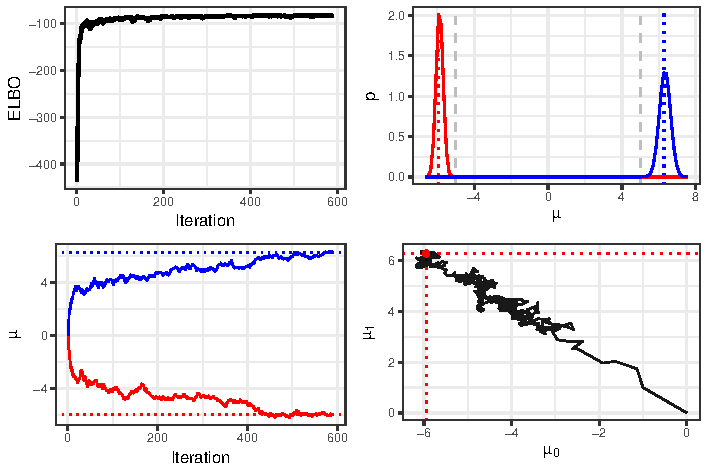
\includegraphics[width=\textwidth]{BBVI_plots.pdf}
    \caption{Example of mean-field variational inference for Bayesian logistic regression.}
    \label{fig:BBVI_plots}
\end{figure}

The posterior predictive distribution of $y^*$ for a new vector of covariates $x^*$ can be approximated using the variational approximation. In particular, we could take $T$ samples from the variational as such: for $j \in \left\{ 1, \ldots, T \right\}$


\begin{enumerate}
  \item Sample a vector $\theta_j \sim q(\theta | \lambda)$
  \item Use that value to sample $y_j^* \sim p(y^* | \theta_j, x^*)$
\end{enumerate}

Then $\left\{ y_j^* \right\}_{j = 1}^T$ is a set of $T$ independent samples from the posterior predictive distribution $\prob{y^* | X, y, x^*}$.

%%%%%%%%%%%%%%%%%%%%%%%%%%%%%%%%%%%%%%%%%%%%%%%%%%%%%%%%%%%%%%%%%%%%%%%%%%%%%%%%%%%%%%%%%%
%%%%%%%%%%%%%%%%%%%%%%%%%%%%%%%%%%%%%%%%%%%%%%%%%%%%%%%%%%%%%%%%%%%%%%%%%%%%%%%%%%%%%%%%%%
%%% ANNs
%%%%%%%%%%%%%%%%%%%%%%%%%%%%%%%%%%%%%%%%%%%%%%%%%%%%%%%%%%%%%%%%%%%%%%%%%%%%%%%%%%%%%%%%%%
%%%%%%%%%%%%%%%%%%%%%%%%%%%%%%%%%%%%%%%%%%%%%%%%%%%%%%%%%%%%%%%%%%%%%%%%%%%%%%%%%%%%%%%%%%

\section{Artificial Neural Networks}

The most basic, and perhaps the best known, type of Artificial Neural Network (ANN) is called a feed-forward neural network or multilayer perceptron (MLP). These models are basically a composition of non-linear functions of the data. We'll first introduce this concept in the ``classical'' way, as they were first introduced. Then we will skip to the Bayesian way.

Let's illustrate the multilayer perceptron with a simple example: consider that we want to model a continuous variable $y$ from a single covariate $x$. A very simple model would be a linear regression, which models each observation $i$ as $y_i = \theta_0 + \theta_1 x_i$, and chooses the values of $\theta_0$ and $\theta_1$ that minimize some error function, most commonly the sum of the squared difference between the real values and the output of the model. ANNs go further and take non-linear transformations of this linear predictor with some function $\sigma(\cdot)$, such that $y_i = \theta_0^{[1]} +  \sum_{j = 1}^m \theta_j^{[1]} \sigma \left( \theta_0^{[0]} + \theta_j^{[0]} x_i \right)$, where $m$ is manually chosen beforehand. A common choice for $\sigma(\cdot)$, which is called the \textbf{activation function}, is the logistic function $\sigma(x) = (1 + e^{-x})^{-1}$
or the hyperbolic tangent $\tanh(\cdot)$. The values of parameters $\theta_k^{[0]}$ and $\theta_k^{[1]}$ for $k \in \left\{ 0, \ldots, m \right\}$ are also chosen to minimize certain error function. Figure \ref{fig:theory_ANN_diagram_01} shows these relationships in a graphic way for a model with $m = 3$ and where we define $a_{k, i} = \sigma \left( \theta_0^{[0]} + \theta_k^{[0]} x_i \right)$ for $k \in \left\{ 1, 2, 3 \right\}$.
This image doesn't explicitly show the parameters $\theta_0^{[0]}$ and $\theta_0^{[1]}$, which are usually called the \textbf{bias} parameters.

\begin{figure}[H]
    \centering
    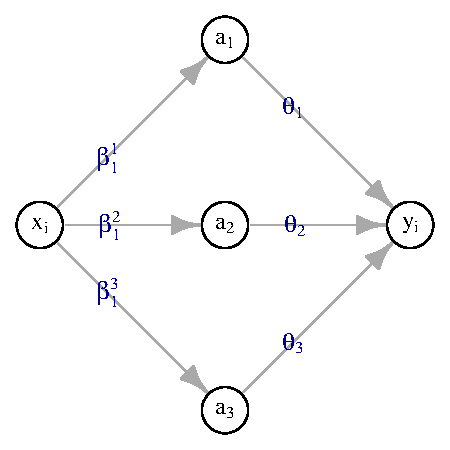
\includegraphics[width=0.5\textwidth]{plot_ANN_01.pdf}
    \caption{Diagram of a multilayer perceptron with $m = 3$.}
    \label{fig:theory_ANN_diagram_01}
\end{figure}

If the response variable $y$ happened to be a categorical variable, let's say binary, then one last transformation would have to be applied to map the model to the $\left[0, 1\right]$ interval and model $y$ as a probability. Then we would have

\begin{equation}
  y_i =
  \phi \left( \theta_0^{[1]} +  \sum_{j = 1}^m \theta_j^{[1]} \sigma \left( \theta_0^{[0]} + \theta_j^{[0]} x_i \right) \right) =
  \phi \left( \theta_0^{[1]} +  \sum_{j = 1}^m \theta_j^{[1]} a_{j,i} \right),
\end{equation}

with $\phi(\cdot)$ the logistic function to map from $\mathbb{R}$ to $\left[ 0, 1 \right]$. The choice of function $\phi(\cdot)$ depends on the nature of the response variable. As we saw previously, in the case of a continuous response variable, $\phi(\cdot)$ is the identity function.

We can establish a more complex model by taking linear combinations of non-linear functions of the previous result. Let's define
\begin{equation}
a_{k,i}^{[1]} = \sigma^{[1]} \left( \theta_{0}^{[1]} + \theta_k^{[0]} x_i \right)
\end{equation}

for $k \in \left\{ 1, \ldots, m \right\}$ and

\begin{equation}
  a_{k,i}^{[2]} = \sigma^{[2]} \left(  \theta_{0,k}^{[1]} + \sum_{j = 1}^m \theta_{j,k}^{[1]} a_{j,1}^{[0]}  \right)
\end{equation}

% \begin{equation}
% a_{k,i}^{[2]} = \theta_0^{j} +  \sum_{k = 1}^m \theta_k^{j} \sigma^{[2)} \left( \theta_0^{k} + \theta_1^{k} x_i \right) =
% \theta_0^{j} +  \sum_{k = 1}^m \theta_k^{j} a_{k,i}^{[1]}
% \end{equation}

for $k \in \left\{ 1, \ldots, r \right\}$, then

\begin{equation}
  y_i = \theta_0^{[2]} + \sum_{j = 1}^r \theta_j^{[2]} a_{j,i}^{[2]}
\end{equation}

where $r$, like $m$, is chosen beforehand. The values $m$ and $r$ are usually called the number of nodes or units of each layer. This is what is called a deeper model, because it has more layers. Notice that we have two different activation functions $\sigma^{[1]}(\cdot)$ and $\sigma^{[2]}(\cdot)$. Each layer can have a different function. The first one could be a sigmoid function and the second one a hyperbolic tangent, or vice versa, or they could both be the same function.

Figure \ref{fig:theory_ANN_diagram_02} shows this graphically with $m = 3$ and $r = 2$. Layers corresponding to $a_{k,i}^{[1]}$ for $k \in \left\{ 1, \ldots, m \right\}$ and $a_{k,i}^{[2]}$ for $k \in \left\{ 1, \ldots, r \right\}$ are called the \textbf{hidden layers}. So figure \ref{fig:theory_ANN_diagram_01} shows a multilayer perceptron with one hidden layer, and figure \ref{fig:theory_ANN_diagram_02} shows a multilayer perceptron with two hidden layers.


\begin{figure}[H]
    \centering
    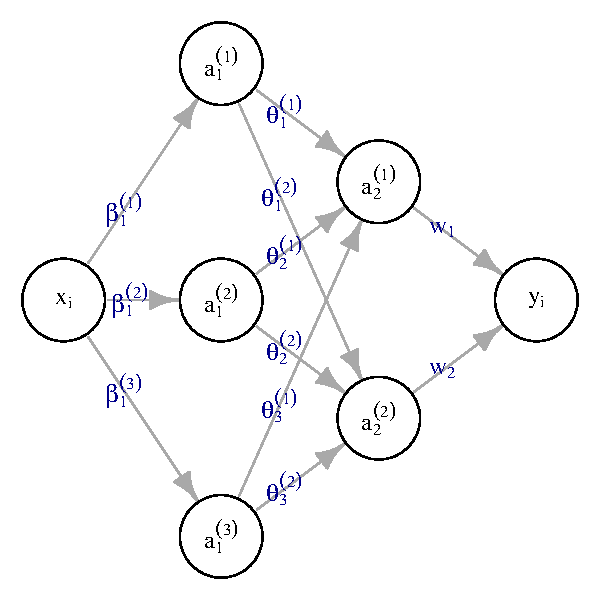
\includegraphics[width=0.6\textwidth]{plot_ANN_02.pdf}
    \caption{Diagram of a multilayer perceptron with two hidden layers, $m = 3$ and $r = 2$.}
    \label{fig:theory_ANN_diagram_02}
\end{figure}

Now that we have a grasp of how the MLP works, we can define it more generally. The notation used will be $y$ for the response variable $n$-dimensional vector, $y_i$ for the $i$-th element of $y$ and $X$ for the data matrix, such that $X \in \mathbb{R}^{n \times p}$, $x_i \in \mathbb{R}^p$ denotes the $i$-th row in $X$ and it represents the values of the covariates for the $i$-th element in the data and $x^{(k)} \in \mathbb{R}^n$ denotes the $k$-th column in $X$ and $x_i^{(k)}$ denotes the $k$-th column-wise element and the $i$-th row-wise element. Since a multilayer perceptron can have any integer number of hidden layers, we will denote the number of layers by $L$, the number of nodes of each layer $l$ by $n^{[l]}$ and the activation function for each layer $l$ by $\sigma^{[l]}(\cdot)$, for $l \in \left\{ 1, \ldots, L \right\}$. The activation function for the last layer will be denoted by $\phi(\cdot)$, as in the binary classification example. The parameter, or weight, that connects the $j$-th node from the $(l-1)$-th layer with the $k$-th node in the $l$-th layer is denoted by $\theta_{j,k}^{[l]}$ and, as before, $a_{k,i}^{[l]}$ denotes the result of the activation function corresponding to the $l$-th layer and the $i$-th observation, for $k \in \left\{ 1, \ldots, n^{[l]} \right\}$; where $\theta_{0,k}^{[l]}$ is the bias term of the $k$-th node in the $l$-th layer. That is,

\begin{equation}
  \label{eq:ann_act_funct_def}
  a_{k,i}^{[l]} = \sigma^{[l]} \left( \theta_{0,k}^{[l-1]} + \sum_{j = 1}^{n^{[l-1]}} \theta_{j,k}^{[l-1]} a_{j,i}^{[l-1]} \right)
\end{equation}

for $k \in \left\{ 1, \ldots, n^{[l]} \right\}$, $j \in \left\{ 1, \ldots, n^{[l-1]} \right\}$, $l \in \left\{ 1, \ldots, L \right\}$ and $i \in \left\{ 1, \ldots, n \right\}$.

To be consistent, $a_{k,i}^{[0]}$ is defined as $x_i^{[k]}$, and so, $a_{k}^{[0]} = x^{(k)} \in \mathbb{R}^n$; and $a_{0,i}^{[0]} = 1$ for all $i \in \left\{ 1, \ldots, n \right\}$, so $a_{0}^{[0]}$ is a vector of ones of dimension $n$ and $n^{[0]}$ is the number of covariates, i.e., $n^{[0]} = p$.

So, in general, a feed-forward neural network or multilayer perceptron with $L$ hidden layers is such that

\begin{equation}
  y_i = \phi \left( \theta_{0,1}^{[L]} +  \sum_{j = 1}^{n^{[L]}} \theta_{j,1}^{[L]} a_{k,i}^{[L]} \right),
\end{equation}

and where equation \ref{eq:ann_act_funct_def} holds. As a way to summarize the whole notation, we will denote a multilayer perceptron with parameters $\Theta$ and data matrix $X$ as $\mathrm{MLP} \left(X, \Theta \right)$, where parameter $\Theta$ is a general way to refer to all parameters $\theta_{j,k}^{[l]}$ for $k \in \left\{ 1, \ldots, n^{[l]} \right\}$, $j \in \left\{ 1, \ldots, n^{[l-1]} \right\}$ and $l \in \left\{ 1, \ldots, L \right\}$.

Figure \ref{fig:theory_ANN_diagram_03} shows an example of an architecture with 2 hidden layers ($L = 2$), 4 covariates ($p = n^{[0]} = 4$), 3 nodes in the first hidden layer ($n^{[1]} = 3$) and 4 nodes in the second hidden layer ($n^{[2]} = 4$).

\begin{figure}[H]
    \centering
    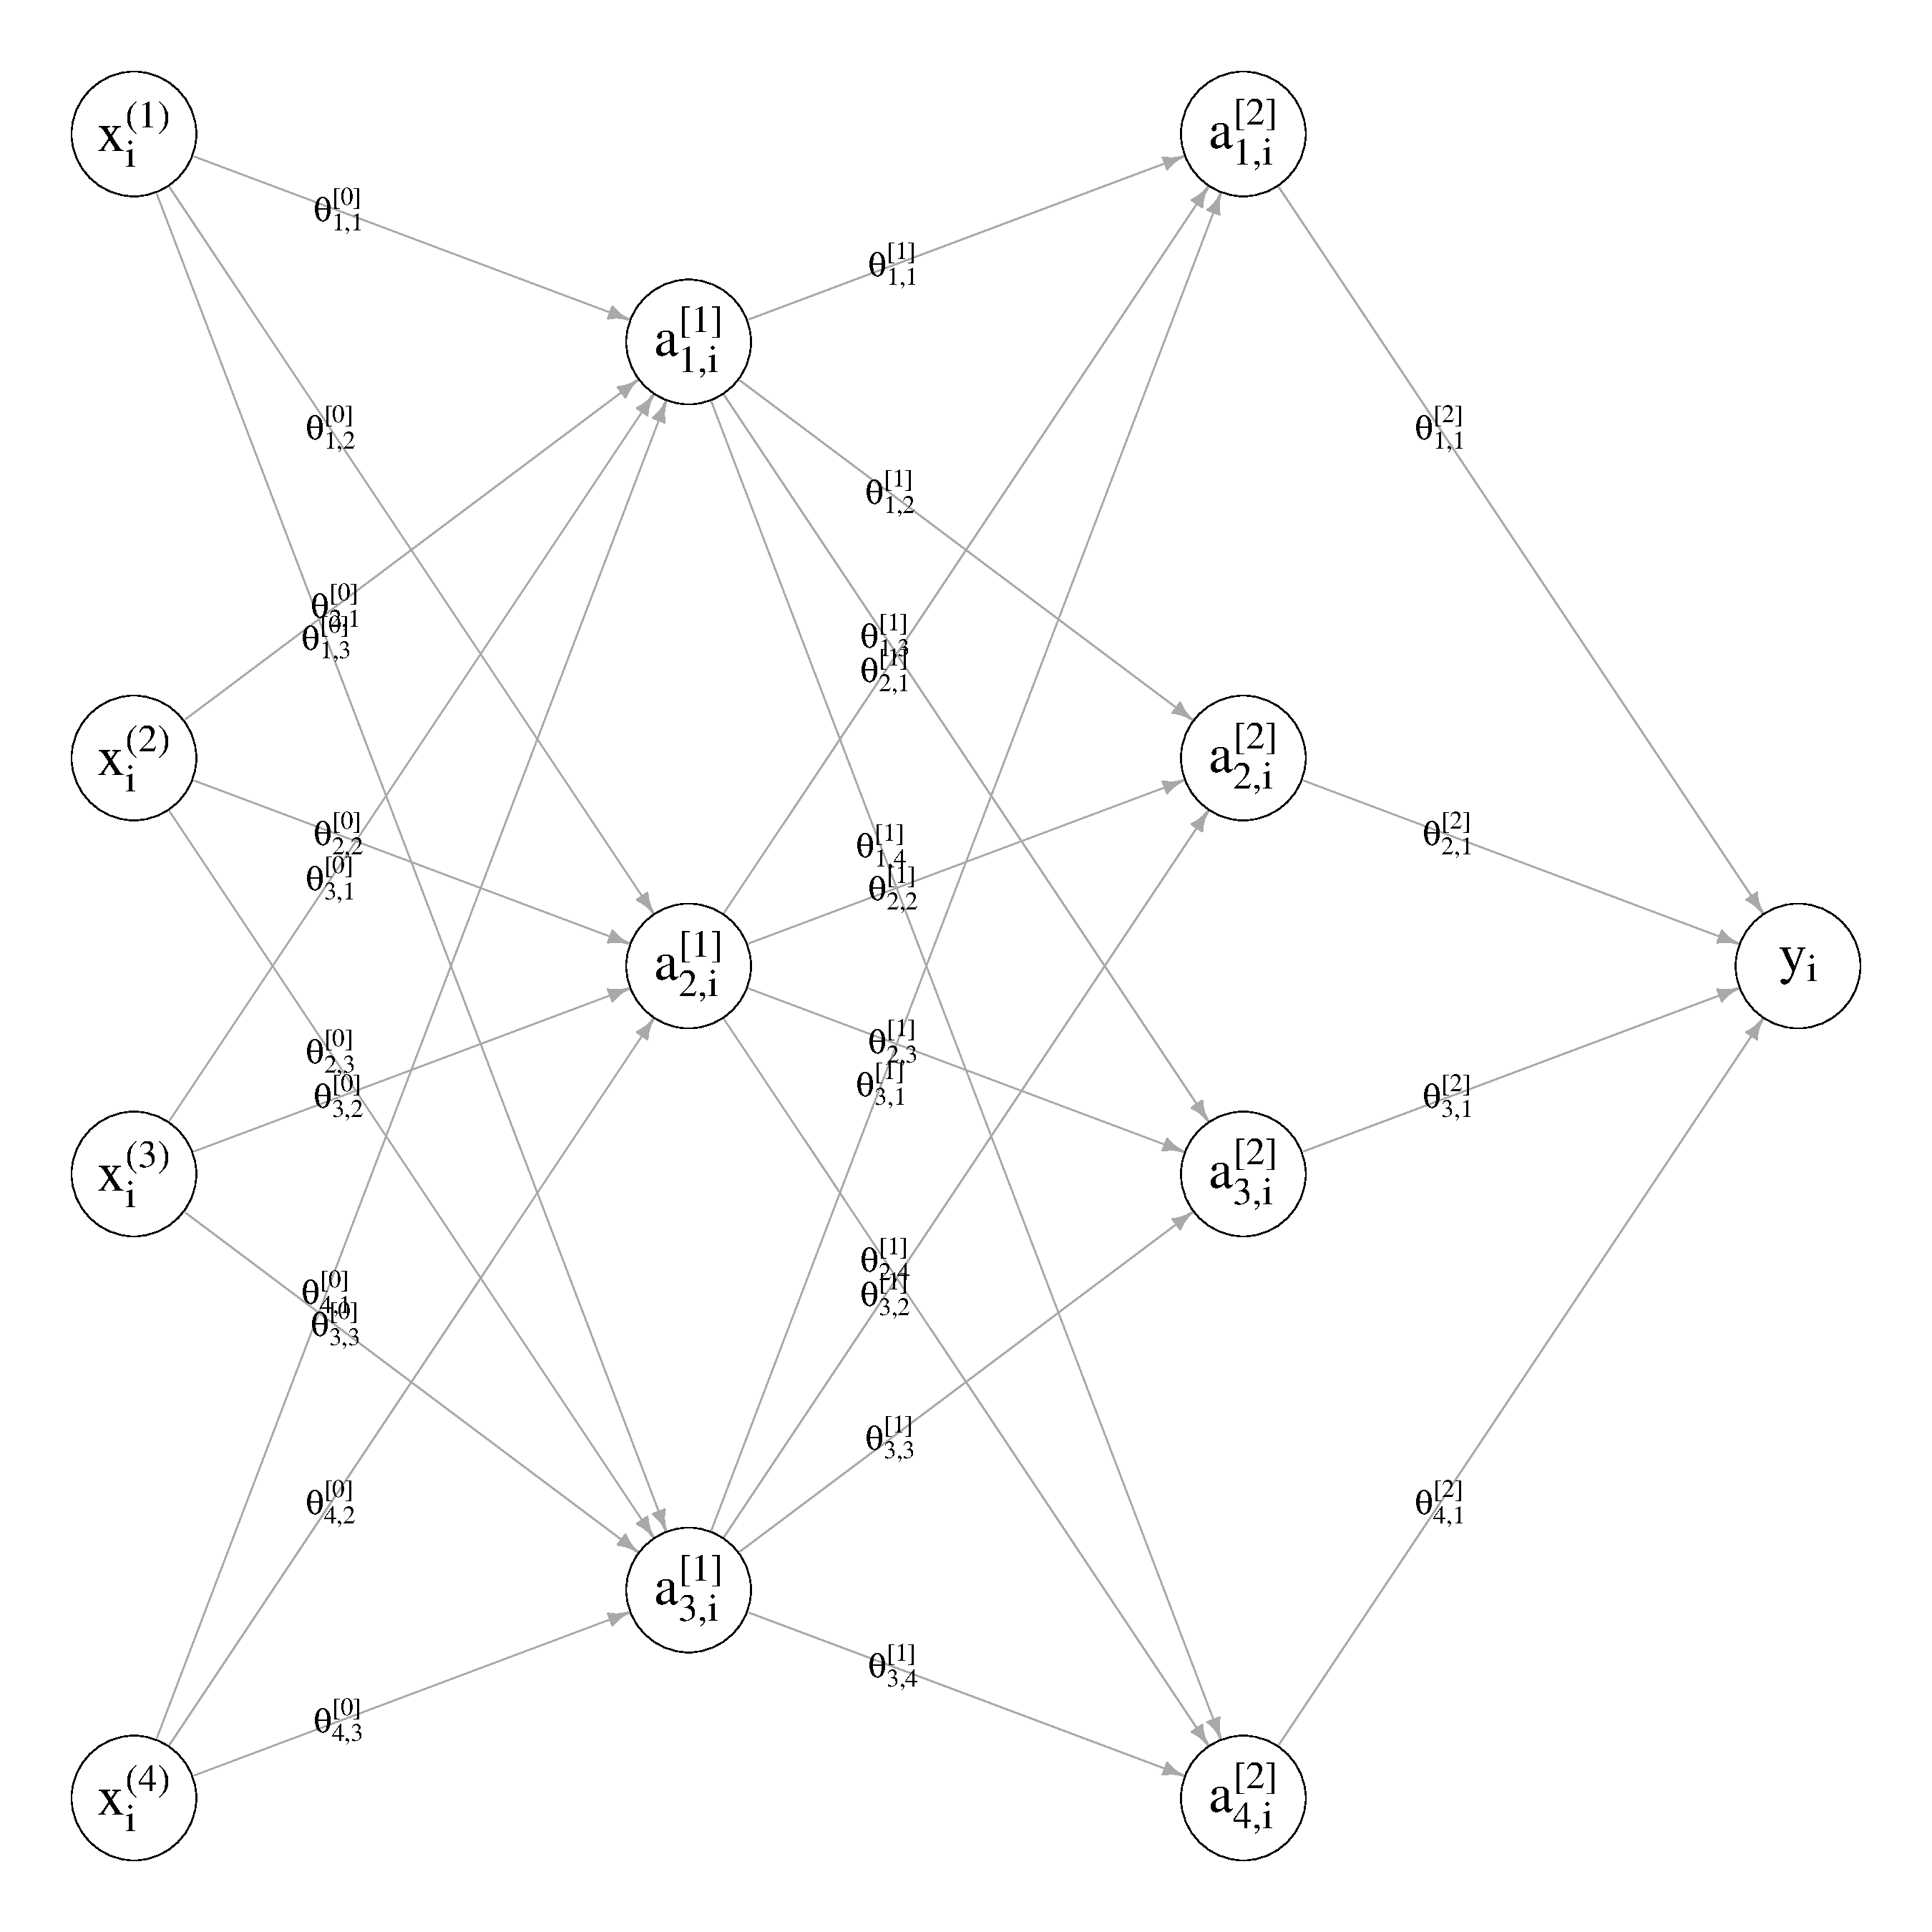
\includegraphics[width=0.95\textwidth]{plot_ANN_03.pdf}
    \caption{Diagram of a multilayer perceptron with two hidden layers using the general notation with $L = 2$, $p = n^{[0]} = 4$, $n^{[1]} = 3$ and $n^{[2]} = 4$.}
    \label{fig:theory_ANN_diagram_03}
\end{figure}

As mentioned before, the values of the parameters in the network are chosen so that they minimize a certain error function. In the continuous case, the commonly called \textbf{squared loss} is often used, defined as the sum of the squared difference between the real values and the output of the model, which is also equivalent to the maximization of a Gaussian likelihood function. This loss function is mathematically defined as

\begin{equation}
  L(\Theta) = \sum_{i = 1}^n \left[ y_i - \hat{y}_i \right]^2
\end{equation}

where $\hat{y_i}$ is the output of the model for the $i$-th observation of the data and the covariate vector $x_i$ and $\Theta$ is the vector of all parameters in the model.

In the case of a binary classification problem, a very commonly used loss is the so-called \textbf{cross-entropy} loss, which is the result of maximizing the log-likelihood of independent Bernoulli response variables. In the context of loss function, it is defined as

\begin{equation}
  \label{eq:binary_cross_entropy_loss}
  L(\Theta) = - \sum_{i = 1}^n \left[ y_i \log{\left( \hat{y}_i \right)} + (1 - y_i) \log{\left( 1 - \hat{y}_i \right)} \right].
\end{equation}

In the case of a multiple classification problem, equation \ref{eq:binary_cross_entropy_loss} is extended for more classes using the same maximum likelihood idea. In a $k$ class classification problem, the loss is defined as

\begin{equation}
  L(\Theta) = - \sum_{i = 1}^n \left[ \sum_{j = 1}^k y_{i,j} \log{\left( \hat{y}_{i,j} \right)}  \right]
\end{equation}

where $y_{i,j} = 1$ if the $i$-th training point belongs to the $j$-th class and $\hat{y}_{i,j}$ is the model's predicted probability of the $i$-th training point belonging to the $j$-th class.

In the Bayesian approach, we first assign prior distributions to each of the parameters and specify a conditional distribution to the response variable $y$. For example, in the continuous case, it is common to assign a Gaussian conditional distribution to $y$, such that

\begin{equation}
  y | \Theta, X \sim \normaldist{\mathrm{MLP}(X, \Theta)}{\sigma^2}
\end{equation}

where $\mathrm{MLP}(X, \Theta)$ denotes the architecture of a multilayer perceptron with parameters $\Theta$ and data matrix $X$. Since the $\Theta$ parameters can be any real value, it is also common to assign a Gaussian distribution to them, so that the prior distribution is such that

\begin{equation}
  \theta_{i,k}^{[l]} \sim \normaldist{\mu_{i,k}^{[l]}}{\sigma_{i,k}^{[l]}}.
\end{equation}

Parameters $\mu_{i,k}^{[l]}$ and $\sigma_{i,k}^{[l]}$ are chosen to reflect the prior knowledge that we may have about the values of the parameters $\theta_{i,k}^{[l]}$. If we have no prior knowledge, then a vague prior can be used.

In contrast to classical neural networks where parameters $\Theta$ are chosen so that they minimize an error function, in Bayesian neural networks we wish to update our knowledge on the parameters $\Theta$ given the data $X$ and $y$. This is achieved with Bayes' theorem in the following way

\begin{equation}
  \prob{\Theta | X, y} = \frac{\prob{y | \Theta, X} \prob{\Theta | X}}{\prob{y | X}}.
\end{equation}

%In our example, $\prob{X | \Theta} = \normalfunc{X}{\mathrm{MLP}(X, \Theta)}{\sigma^2}$ and $\prob{\Theta} = \normalfunc{\Theta}{[]}$
In our example, $\prob{y | \Theta, X}$ and $\prob{\Theta | X}$ are the joint density functions of Gaussian random variables with their corresponding parameter values.

To make predictions in the Bayesian case, we use the posterior predictive distribution defined in equation \ref{eq:post_pred_dist}.


%%%%%%%%%%%%%%%%%%%%%%%%%%%%%%%%%%%%%%%%%%%%%%%%%%%%%%%%%%%%%%%%%%%%%%%%%%%%%%%%%%%%%%%%%%
%%%%%%%%%%%%%%%%%%%%%%%%%%%%%%%%%%%%%%%%%%%%%%%%%%%%%%%%%%%%%%%%%%%%%%%%%%%%%%%%%%%%%%%%%%
%%% CNNs
%%%%%%%%%%%%%%%%%%%%%%%%%%%%%%%%%%%%%%%%%%%%%%%%%%%%%%%%%%%%%%%%%%%%%%%%%%%%%%%%%%%%%%%%%%
%%%%%%%%%%%%%%%%%%%%%%%%%%%%%%%%%%%%%%%%%%%%%%%%%%%%%%%%%%%%%%%%%%%%%%%%%%%%%%%%%%%%%%%%%%

\section{Convolutional Neural Networks}

Convolutional Neural Networks (CNNs) are neural networks with a quite particular architecture and are widely used in computer vision problems, such as image classification or object detection in a video. They were introduced by \citeauthor{lecun1989generalization} in \citeyear{lecun1989generalization} as a way to constrain the number of parameters needed to perform automatic image classification \cite{lecun1989generalization}. The main idea is that in images, pixels close to each other tend to be similar, whereas pixels far away from each other tend to be different. This notion of proximity is used by CNN's architecture, and leverages three concepts: sparse interactions, parameter sharing and equivariant representations \cite[p.~335]{bengio2015deep}.

\begin{itemize}
  \item Sparse interactions: In MLPs, every unit is connected to all other units in the next layer, but in CNNs, only a small number of units is connected to another small number of units. This means fewer parameters and, hence, less memory usage and faster computation.
  \item Parameter sharing: Different units share the same set of parameters. The same convolution is used many times in the image and, thus, the number of parameters is further reduced.
  \item Equivariant representations: The architecture of CNNs provides equivariance in translations, meaning that if the input is changed, the output is changed in the same fashion. For example: in an image, if an object is moved in the input, its representation will be moved in the same way in the output.
\end{itemize}

\subsection{Convolution operation}

The base of CNNs is the convolution operation, which will be described assuming an image. Let's assume that we have an image represented as a $m \times n$ matrix $I$, with $I_{i,j}$ represents the pixel in the $i$-th row and $j$-th column as such

\begin{equation}
  I =
    \begin{bmatrix}
      I_{1,1} & I_{1,2} & I_{1,3} & \dots  & I_{1,n} \\
      I_{2,1} & I_{2,2} & I_{2,3} & \dots  & I_{2,n} \\
      \vdots & \vdots & \vdots & \ddots & \vdots \\
      I_{m,1} & I_{m,2} & I_{m,3} & \dots  & I_{m,n}
    \end{bmatrix}.
\end{equation}

The convolution operation uses another matrix called a \textbf{filter} or a \textbf{kernel}, with dimensions $p \times r$. This matrix must be of a lower dimension than the image, that is, $p < m$ and $r < n$. Let's denote the filter as matrix $K$ as such

\begin{equation}
  K =
    \begin{bmatrix}
      \theta_{1,1} & \theta_{1,2} & \theta_{1,3} & \dots  & \theta_{1,q} \\
      \theta_{2,1} & \theta_{2,2} & \theta_{2,3} & \dots  & \theta_{2,q} \\
      \vdots & \vdots & \vdots & \ddots & \vdots \\
      \theta_{p,1} & \theta_{p,2} & \theta_{p,3} & \dots  & \theta_{p,q}
    \end{bmatrix}.
\end{equation}

The convolution operation between $I$ and $K$ is denoted as $I * K$, and its result is another matrix $S$, for which each element is defined as

\begin{equation}
  \label{eq:2d_conv_def}
  S_{i,j} = (I * K)_{i,j} = \sum_{k} \sum_{l} I_{i+k-1,j+l-1} K_{k, l}.
\end{equation}

An example of this is shown in figure \ref{fig:conv_example}, in which $I$ is a $7 \times 7$ image matrix and the kernel is a $3 \times 3$ matrix. The result is a $5 \times 5$ matrix in which element is computed using equation \ref{eq:2d_conv_def}. For instance, the element on the first row and fourth column of the result matrix, that is, $S_{1,4}$ is computed as

\begin{equation}
  \begin{split}
      S_{1,4} & =
      \sum_{k=1}^3 \sum_{l=1}^3 I_{1+k-1,4+l-1} K_{k, l} \\
      & = I_{1,4}K_{1,1} + I_{1,5}K_{1,2} + I_{1,6}K_{1,3} \\
      & + I_{2,4}K_{2,1} + I_{2,5}K_{2,2} + I_{2,6}K_{2,3} \\
      & + I_{3,4}K_{3,1} + I_{3,5}K_{3,2} + I_{3,6}K_{3,3} \\
      & = ( 1 \times 1 ) + ( 0 \times 0 ) + ( 0 \times 1 ) \\
      & + ( 1 \times 0 ) + ( 1 \times 1 ) + ( 0 \times 0 ) \\
      & + ( 1 \times 1 ) + ( 1 \times 0 ) + ( 1 \times 1 ) \\
      & = 4.
  \end{split}
\end{equation}

The rest of the elements are computed in a similar way. Note that the resulting matrix is smaller than the original image matrix. Also note, that the convolution kernel in the example only has 9 parameters which are used by the whole image matrix, and these parameters are usually estimated with data.

Note that an image classification problem could be solved by turning the input image into a long vector, but then this would be fed to a fully connected layer, which would mean that a large number of parameters would have to be fit. This is one of the reason convolutions are used: instead of estimating a large number of parameters, the convolution operation needs a small number of parameters (9 in the case of the example) to be fit. Additionally, the convolution operation takes into account the topology of the image input, which have a very local structure \cite{lecun1998gradient}.

% \begin{equation}
%   S_{1,4} = \sum_{k=1}^3 \sum_{l=1}^3 I_{1+k-1,4+l-1} K_{k, l} = I_{1,4}K_{1,1} + I_{1,5}K_{1,2} + I_{1,6}K_{1,3} + I_{2,4}K_{2,1} + I_{2,5}K_{2,2} + I_{2,6}K_{2,3} + I_{3,4}K_{3,1} + I_{3,5}K_{3,2} + I_{3,6}K_{3,3}
% \end{equation}

\begin{figure}[H]
    \centering
    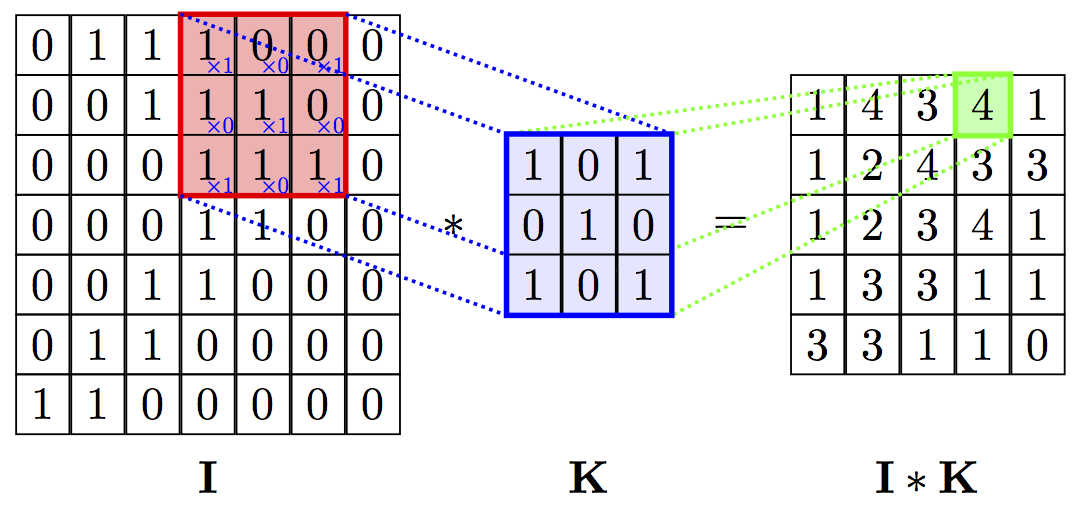
\includegraphics[width=0.9\textwidth]{convolution_example.png}
    \caption{Example of a convolution operation. Source: \url{https://github.com/PetarV-/TikZ}}
    \label{fig:conv_example}
\end{figure}

\subsection{Pooling}

When using CNNs, a pooling layer is also usually added after each convolutional layer. This pooling layer summarizes adjacent pixels, and it is used because it helps to achieve invariance and reduce the image of the output so that there are fewer parameters in the next layers \cite{bengio2015deep}. A very commonly used pooling function is \textbf{max pooling}, which returns the maximum value of a neighborhood of pixels. An example of max pooling is shown in figure \ref{fig:max_pool_example} for a $4 \times 4$ matrix, resulting in a $2 \times 2$ matrix after the function is applied.

\begin{figure}[H]
    \centering
    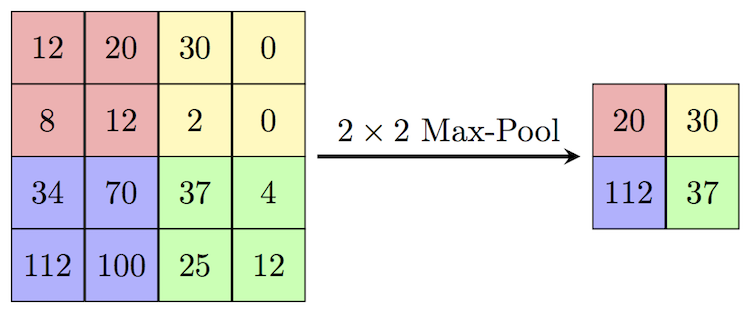
\includegraphics[width=0.6\textwidth]{max_pool_example.png}
    \caption{Example of max pooling function. Source: \url{https://computersciencewiki.org/index.php/File:MaxpoolSample2.png}}
    \label{fig:max_pool_example}
\end{figure}


\subsection{Architecture example}

To illustrate how all these concepts are put together, we will show an example of an architecture that is very commonly used in image classification problems, called \textbf{LeNet architecture}, introduced by \citeauthor{lecun1998gradient} in \citeyear{lecun1998gradient} for a digit classification problem \cite{lecun1998gradient}. The architecture assumes a grayscale input image of $32 \times 32$ pixels, which is then fed to 6 convolutional filters of size $5 \times 5$, each followed by an activation function and a $2 \times 2$ max pooling layer, then 16 convolutional filters of size $5 \times 5$, each with their corresponding activation functions and then the $2 \times 2$ max pooling layer, followed by two fully connected layers of sizes 120 and 84, and finally a softmax transformation to map to the 10 digit classification problem probabilities.

\begin{figure}[H]
    \centering
    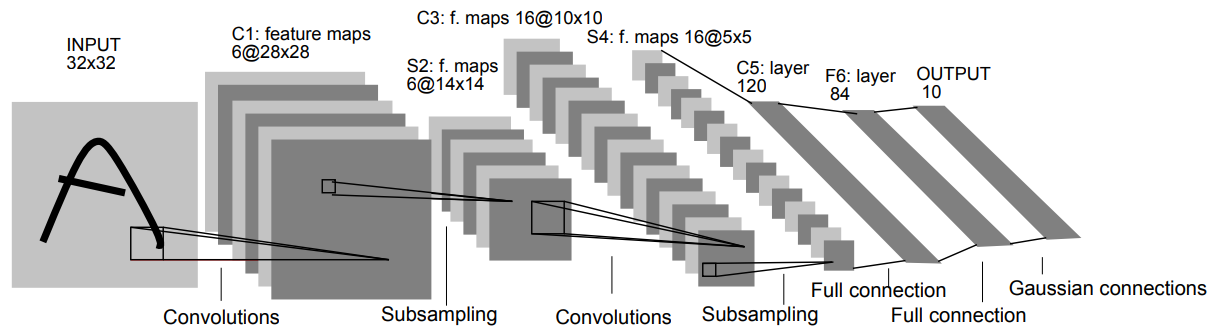
\includegraphics[width=\textwidth]{lenet.png}
    \caption{LeNet architecture (picture taken from \cite{lecun1998gradient}). The feature maps correspond to the convolutional filters and the subsampling refers to max pooling.}
    \label{fig:lenet_architecture}
\end{figure}



%%%%%%%%%%%%%%%%%%%%%%%%%%%%%%%%%%%%%%%%%%%%%%%%%%%%%%%%%%%%%%%%%%%%%%%%%%%%%%%%%%%%%%%%%%
%%%%%%%%%%%%%%%%%%%%%%%%%%%%%%%%%%%%%%%%%%%%%%%%%%%%%%%%%%%%%%%%%%%%%%%%%%%%%%%%%%%%%%%%%%
%%% AL
%%%%%%%%%%%%%%%%%%%%%%%%%%%%%%%%%%%%%%%%%%%%%%%%%%%%%%%%%%%%%%%%%%%%%%%%%%%%%%%%%%%%%%%%%%
%%%%%%%%%%%%%%%%%%%%%%%%%%%%%%%%%%%%%%%%%%%%%%%%%%%%%%%%%%%%%%%%%%%%%%%%%%%%%%%%%%%%%%%%%%

\section{Active Learning}

An active learning problem is one in which the learner selects its own training data. For example, in a supervised learning problem where we are given a data set with covariates $X$ and response variable $y$. First we train a model $\hat{f}$ with the data that we have, afterwards the learner can choose new data $x^*$ from an unlabeled pool of data, ask to an \textit{oracle} what the corresponding output $y^*$ is, and then add the pair $(x^*, y^*)$ to the training data. The main goal of active learning is to select which $x^*$ to incorporate to the training data \cite{cohn1996active}.

The new example is chosen using an \textbf{acquisition function} $a(x, \hat{f})$ that is usually based on the model's uncertainty about the prediction. The new observation $x^*$ is chosen so that it maximizes the acquisition function of all the observations in the pool set. In practice, the oracle is usually a human that gives the corresponding label $y^*$. After the new observation is added to the training data, the model is retrained with the updated data set. This process is iteratively repeated, with the training set increasing in size with every iteration. In the end, it is expected that this procedure leads to a better predictive performance than randomly selecting new observations to add to the training data.

The acquisition functions that will be used and compared in this work are four, and three of them use the posterior predictive distribution, particularly, the posterior predictive probability of an observation $x^*$ having a label $y^*$ belonging to a class $c$, denoted as  $p(y^* = c | X, y, x^*)$. Naturally, because of the definition of these acquisition functions, they only work in classification frameworks.

\begin{enumerate}
  \item Predictive entropy:

  $ \mathbb{H} \left[ y^* | X, y, x^* \right] = - \sum_c p(y^* = c | X, y, x^*) \log p(y^* = c | X, y, x^*)$.

  \item Bayesian Active Learning by Disagreement (BALD):

  $ \mathbb{H} \left[ y^* | X, y, x^* \right] - \mathbb{E}_{p(\theta | X, y)} \left[ \mathbb{H} \left[ y^* | x^*, \theta \right] \right]$.

  \item Variation ratios: $1 - \max_y p(y^* | X, y, x^*)$.

  \item Random: Choosing an observation uniformly random from the pool of unlabeled data.

\end{enumerate}





























%%%%%%%%%%%%%%%%%%%%%%%%%%%%%%%%%%%%%%%%%%%%%%%%%%%%%%%%%%%%%%%%%%%%%%%%%%%%%%%%%%%%%%%%%%
%%%%%%%%%%%%%%%%%%%%%%%%%%%%%%%%%%%%%%%%%%%%%%%%%%%%%%%%%%%%%%%%%%%%%%%%%%%%%%%%%%%%%%%%%%
%%% end
%%%%%%%%%%%%%%%%%%%%%%%%%%%%%%%%%%%%%%%%%%%%%%%%%%%%%%%%%%%%%%%%%%%%%%%%%%%%%%%%%%%%%%%%%%
%%%%%%%%%%%%%%%%%%%%%%%%%%%%%%%%%%%%%%%%%%%%%%%%%%%%%%%%%%%%%%%%%%%%%%%%%%%%%%%%%%%%%%%%%%


	%!TEX root = ../msc_thesis.tex

\chapter{Experimental results}
\label{ch:results}

In this section, the results of the experiments run are shown. Everything was done in Keras using Tensorflow as backend and mainly through R, although some Python code was used via the \texttt{reticulate} package.

\section{MNIST dataset}

The first goal was to replicate \citeauthor{Gal2016Active}'s work done with MNIST dataset in \citetitle{Gal2016Active}. The results can be seen in figure \ref{fig:mnist_comparison_active_learning_random}, where I compare my results (on the left) with the original paper's results (right). The results are pretty similar overall, although the mean STD acquisition function was not implemented in the replication due to the bad performance shown in the paper.

Even when my implementation achieved the goal of outperforming a random acquisition function, when comparing Bayesian and frequentist approaches the results differ. The paper's authors claim that the use of a Bayesian approach in the acquisition process of Active Learning leads to better accuracy with fewer images, but in my implementation there is virtually no distinction between both approaches. This can be seen in figures in \ref{fig:mnist_pred_entropy_AL} and \ref{fig:mnist_var_ratios_AL} that show my results (left) and the paper's authors results (right). In the paper, the frequentist acquisition functions show a worse performance than their Bayesian counterparts, but in my implementation there is no distinction. For example, with predictive entropy in figure \ref{fig:mnist_pred_entropy_AL}, the frequentist acquisition function in the original paper achieve a 90\% accuracy with around 300 images, while in my implementation this accuracy is first achieved with around 200 images.


\begin{figure}[H]
    \centering
    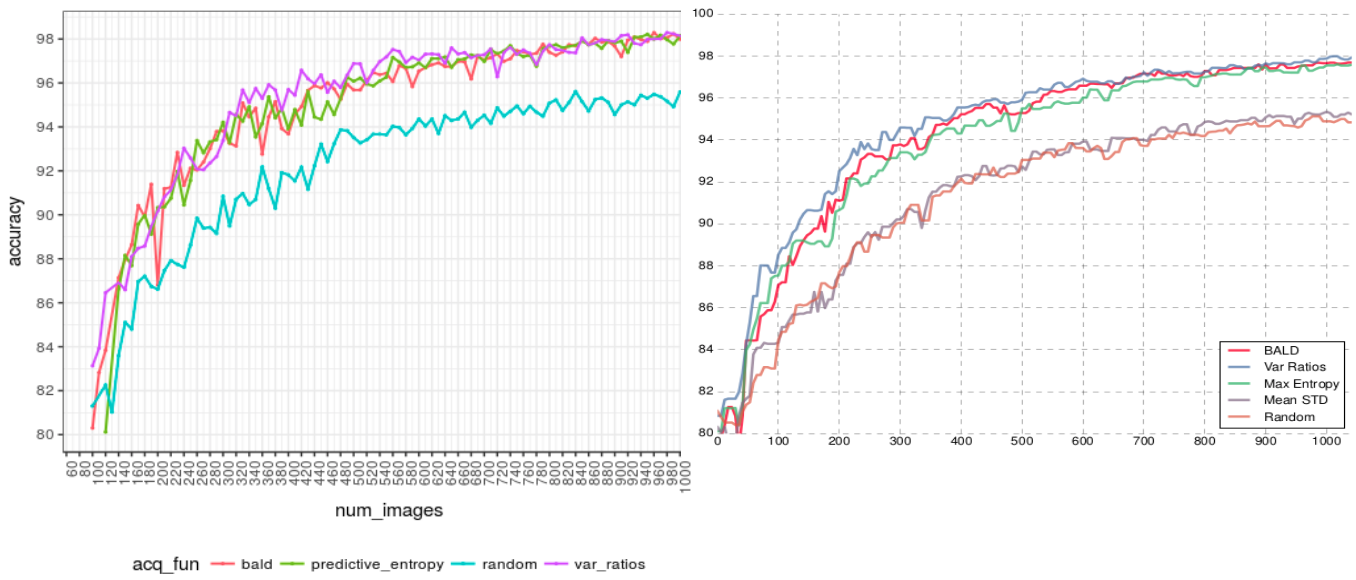
\includegraphics[width=\textwidth]{mnist_bayesian_accuracy.png}
    \caption{Accuracy of models in each acquisition step. The left picture shows my implementation and the right picture shows \citeauthor{Gal2016Active}'s implementation.}
    \label{fig:mnist_comparison_active_learning_random}
\end{figure}

\begin{figure}[H]
  \centering
  \subfloat[My results.]{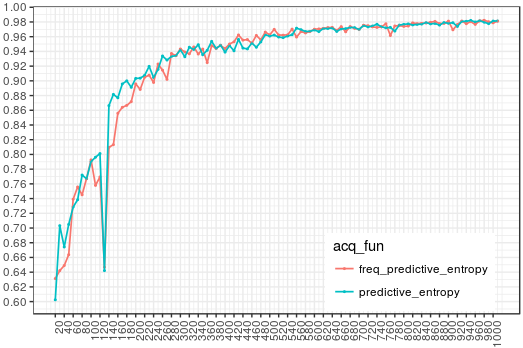
\includegraphics[width=0.5\textwidth]{mnist_pred_entropy_mine.png}}
  \hfill
  \subfloat[Paper's results.]{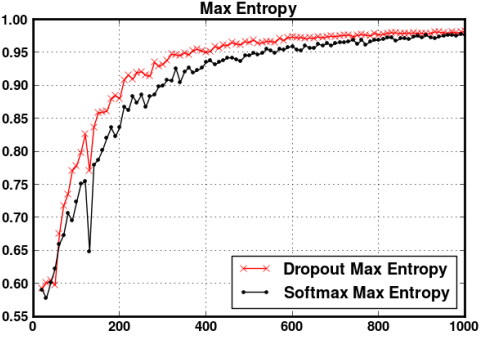
\includegraphics[width=0.5\textwidth]{mnist_pred_entropy_islam.png}}
  \caption{Accuracy of Bayesian and frequentist models in each acquisition step using predictive entropy as acquisition function. The left picture shows my implementation and the right picture shows \citeauthor{Gal2016Active}'s implementation.}
  \label{fig:mnist_pred_entropy_AL}
\end{figure}


\begin{figure}[H]
  \centering
  \subfloat[My results.]{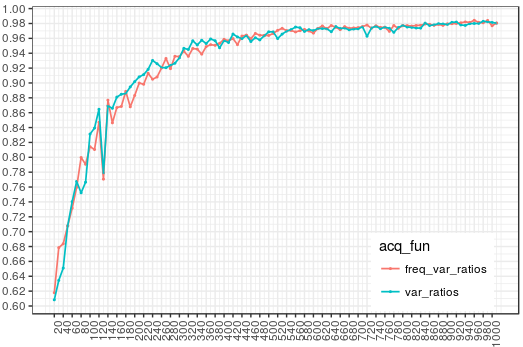
\includegraphics[width=0.5\textwidth]{mnist_var_ratio_mine.png}}
  \hfill
  \subfloat[Paper's results.]{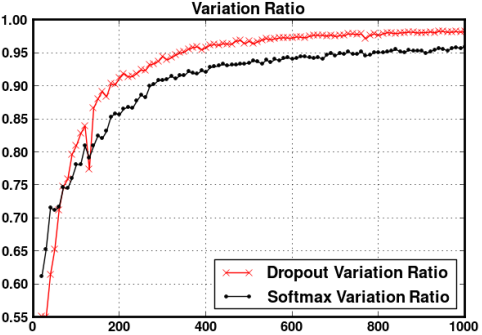
\includegraphics[width=0.5\textwidth]{mnist_var_ratio_islam.png}}
  \caption{Accuracy of Bayesian and frequentist models in each acquisition step using variation ratios as acquisition function. The left picture shows my implementation and the right picture shows \citeauthor{Gal2016Active}'s implementation.}
  \label{fig:mnist_var_ratios_AL}
\end{figure}

One more thing that should be mentioned is that I could not implement the BALD acquisition in the frequentist setting because of the way it is defined. The BALD uncertainty for a prediction $y$ given model parameters $\mathcal{W}$, features $x$ and training data $\mathcal{D}$ is defined as

\begin{equation}
	\label{eq:bald_def}
	\mathbb{I}[y, \mathcal{W} | x, \mathcal{D}] = \mathbb{H}[y | x, \mathcal{D}] - \mathbb{E}_{p(\mathcal{W} | \mathcal{D})}[\mathbb{H}[y | x, \mathcal{W}]]
\end{equation}

with $\mathbb{H}[y | x, \mathcal{D}]$ is the predictive entropy and is defined as $-\sum_c p(y = c | x, \mathcal{D}) \log p(y = c | x, \mathcal{D})$. In the Bayesian case, we have a set of $T$ dropout samples that approximate the predictive distribution, so the second part of equation \ref{eq:bald_def}, i.e., the expected value $\mathbb{E}_{p(\mathcal{W} | \mathcal{D})}[\mathbb{H}[y | x, \mathcal{W}]]$ is approximated by averaging the predictive entropy of each predictive sample; this way $\mathbb{I}[y, \mathcal{W} | x, \mathcal{D}]$ is computed by taking the difference of this quantity and the first part of equation \ref{eq:bald_def}. In the frequentist case, we only have one point estimate, so that difference is zero, so $\mathbb{I}[y, \mathcal{W} | x, \mathcal{D}]$ is zero for all points in the pool set. To this day, I don't know how the paper's authors computed it because their Github code is not clear and they haven't answered my email where I asked them that.

\section{Cats and dogs dataset}


\begin{figure}[H]
    \centering
    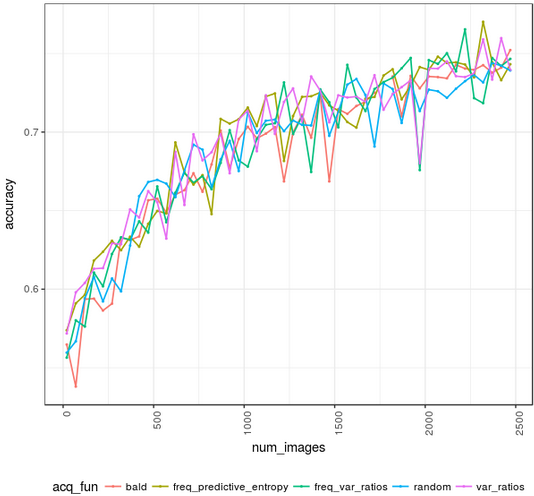
\includegraphics[width=\textwidth]{cats_dogs_accuracy.png}
    \caption{Accuracy of models in each acquisition step in the cats and dogs dataset.}
    \label{fig:cats_dogs_comparison_active_learning_random}
\end{figure}


\section{CIFAR10 dataset}

\begin{figure}[H]
    \centering
    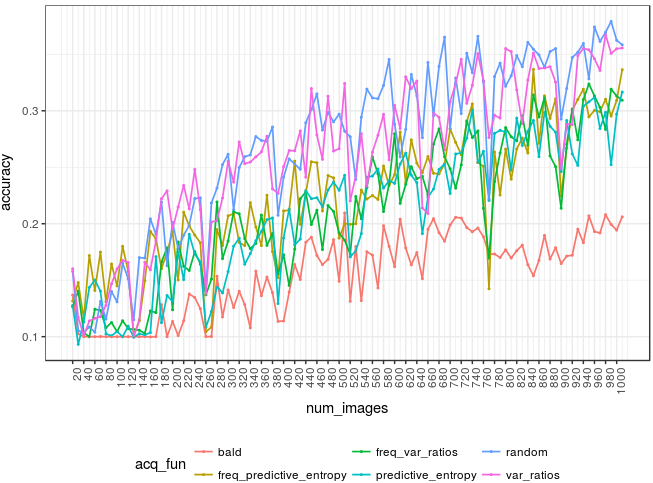
\includegraphics[width=\textwidth]{cifar10_accuracy.png}
    \caption{Accuracy of models in each acquisition step in the CIFAR10 dataset.}
    \label{fig:cifar10_comparison_active_learning_random}
\end{figure}

\section{Discussion}

\begin{figure}[H]
    \centering
    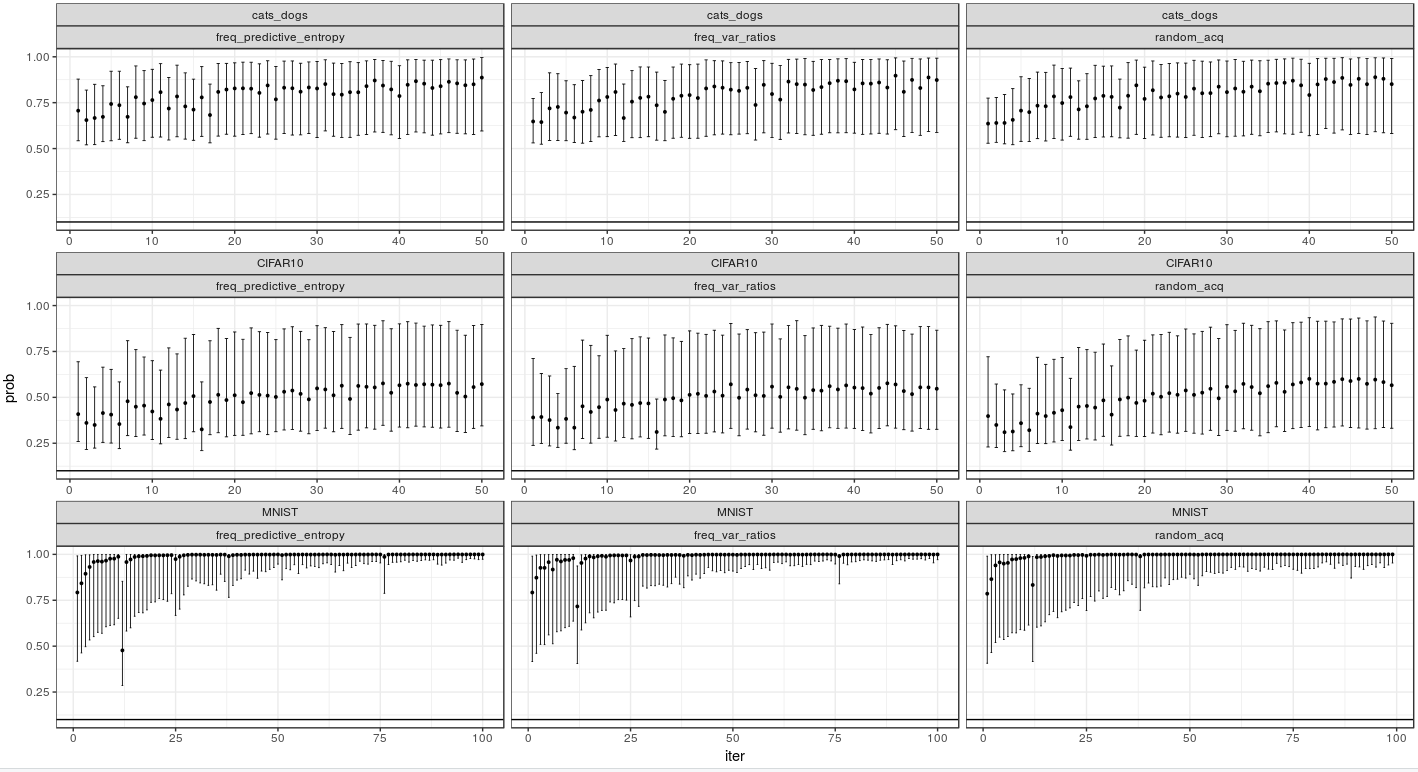
\includegraphics[width=\textwidth]{probs_iterations.png}
    \caption{Probabilities of each model in each acquisition iteration.}
    \label{fig:probs_iterations}
\end{figure}


	%!TEX root = ../mbc_msc_thesis.tex

\chapter{Conclusions and future work}
\label{ch:conclusions}

Wow. Such conclusions. Very science. So smrt.





	%%%%%%%%%%%%%%%%%%%%%%%%%%%%%%%%%%%%%%%%%%%%%%
	% APPENDIX
	%%%%%%%%%%%%%%%%%%%%%%%%%%%%%%%%%%%%%%%%%%%%%%
	\appendix
	% \include{Chapters/appendixA}

	%%%%%%%%%%%%%%%%%%%%%%%%%%%%%%%%%%%%%%%%%%%%%%
	% BIBLIOGRAPHY
	%%%%%%%%%%%%%%%%%%%%%%%%%%%%%%%%%%%%%%%%%%%%%%
	\clearpage
	\addcontentsline{toc}{chapter}{References}



\begingroup
\raggedright
\sloppy
\printbibliography
\endgroup

% \nocite{*}

\end{document}

%%% Local Variables:
%%% mode: latex
%%% TeX-master: t
%%% End:
